\documentclass[a4paper, 11pt]{scrartcl}

% font, language
\usepackage[utf8]{inputenc}
\usepackage[T1]{fontenc}
\usepackage{lmodern}

\usepackage{float}
\usepackage{longtable}

\usepackage{scrextend}

% quoting
\usepackage{quoting, xparse}
\usepackage[hyphens]{url}

\usepackage[toc,page]{appendix}

% highliting
\usepackage{color,soul}

\usepackage[dvipsnames]{xcolor}

\usepackage{svg}
\usepackage{rotating}
\usepackage{ctable} % for \specialrule command
\usepackage{tabularx}

\NewDocumentCommand{\bywhom}{m}{% the Bourbaki trick
  {\nobreak\hfill\penalty50\hskip1em\null\nobreak
   \hfill\mbox{\normalfont(#1)}%
   \parfillskip=0pt \finalhyphendemerits=0 \par}%
}

\NewDocumentEnvironment{pquotation}{m}
  {\begin{quoting}[
     indentfirst=true,
     leftmargin=\parindent,
     rightmargin=\parindent]\itshape}
  {\bywhom{#1}\end{quoting}}

\usepackage{todonotes}
\usepackage{caption}
\newcommand{\source}[1]{\caption*{\hfill Source: {#1}} }

\usepackage{fontspec}
\setmainfont{Latin Modern Roman}

\usepackage{polyglossia}
\setmainlanguage[babelshorthands=true]{german}
\setdefaultlanguage[spelling=new]{german}
\usepackage[autostyle]{csquotes}
\MakeAutoQuote{»}{«}

\usepackage{enumitem}

% graphics
\usepackage{graphicx}
\graphicspath{ {images/} }

% code highlighting
\usepackage{listings}
\usepackage{color}
%\lstset{ % General setup for the package
%	language=java
%}

\lstset{
	%basicstyle=\scriptsize\sffamily\color{black},
	frame=single,
	numbers=left,
	numbersep=5pt,
	numberstyle=\tiny\color{gray},
	showspaces=false,
	showstringspaces=false,
	tabsize=1
}

\usepackage{listings}
\lstdefinelanguage{Kotlin}{
	comment=[l]{//},
	commentstyle={\color{gray}\ttfamily},
	emph={delegate, filter, first, firstOrNull, forEach, lazy, map, mapNotNull, println, return@},
	emphstyle={\color{OrangeRed}},
	identifierstyle=\color{black},
	keywords={abstract, actual, as, as?, break, by, class, companion, continue, data, do, dynamic, else, enum, expect, false, final, for, fun, get, if, import, in, interface, internal, is, null, object, override, package, private, public, return, set, super, suspend, this, throw, true, try, typealias, val, var, vararg, when, where, while},
	keywordstyle={\color{NavyBlue}\bfseries},
	morecomment=[s]{/*}{*/},
	morestring=[b]",
	morestring=[s]{"""*}{*"""},
	ndkeywords={@Deprecated, @JvmField, @JvmName, @JvmOverloads, @JvmStatic, @JvmSynthetic, Array, Byte, Double, Float, Int, Integer, Iterable, Long, Runnable, Short, String},
	ndkeywordstyle={\color{BurntOrange}\bfseries},
	sensitive=true,
	stringstyle={\color{ForestGreen}\ttfamily},
}

% toc depth
\setcounter{tocdepth}{4}
\setcounter{secnumdepth}{4}

% bib
\usepackage[
	backend=biber,
	sorting=none
]{biblatex}

\addbibresource{references/references.bib}
\usepackage{hyperref}
\usepackage{xcolor}
\hypersetup{
	colorlinks,
	linkcolor={red!0!black},
	citecolor={blue!70!black},
	urlcolor={blue!70!black}
}

\usepackage{enumitem}
\setlist[enumerate]{label*=\arabic*.}

% title, author
\title{Bachelor-Thesis}
\author{Roman Quistler}

\begin{document}
	
	
	
	% \begin{titlepage}
	\centering
	
\includegraphics[width=0.30\textwidth]{hsb_logo.png}
	\par\vspace{1cm}
	{\scshape\LARGE Hochschule Bremen \par}
	\vspace{1cm}
	{\scshape\Large Bachelorarbeit  \par}
	\vspace{1.5cm}
	{\LARGE\bfseries Entwicklung eines Model-View-Intent Framework für die Plattform Android\par}
	\vspace{0.5cm}
	{\normalsize\itshape Medieninformatik B.Sc. \par}
	\vspace{2cm}
	{\Large\itshape Roman Quistler \par}
	\vfill
	\vfill
	{\large\today\par}
\end{titlepage}
	
	\pagenumbering{gobble}
	\newpage
	\tableofcontents
	\newpage
	\pagenumbering{arabic}
	
	\newpage
	
%	\section{Einleitung}
\label{sec:einleitung}

Bis zum Jahre 1973 und der Entwicklung des ersten Eingabegerätes mit Graphischer Oberfläche (GUI) (Xerox Alto \cite{xeroxAlto}) erfolgte die Interaktion mit einem Computer im Wesentlichen über eine Konsole. Dies reduzierte die Ein- und Ausgabe eines Programms auf rein textuelle Elemente. Seither hat sich viel getan: Die Erschaffung des Internets leitet den Beginn von Webseiten ein, welche von einer anfänglich statischen Ausprägung zu der heutigen dynamisch und komplexen wuchsen. Dazu gesellten sich im Laufe der Zeit mobile Endgeräte - zu Beginn bestückt mit Tasten für die Eingabe, sowie einem primitiven Bildschirm für die Anzeige finden sich heutzutage vorwiegend leistungsfähige, auf einem kapazitiven Touchscreen basierende Smartphones wieder. Hierbei ist über die Jahre der Funktionsumfang von Betriebssystem und Applikationen im Allgemeinen gestiegen.

\subsection{Problemfeld}
\label{subsec:problemfeld}
Die Herausforderung für einen Entwickler ist es, die Nutzerschnittstelle (auch: »Presenation Layer« \cite{presentationLayerpatternsOfEnterpriseApplicationArchitectureMartinFowler}),
innerhalb einer »Drei-Schichtenarchitektur«
\cite{threeTierArchitectureDonaldWolfe2013}
sinnvoll aufzubauen und dabei die Modellierung und Verwaltung des Zustandes innerhalb einer Applikation zu berücksichtigen. Hierfür müssen auch externe Vorkommnisse wie bspw.. die Aktualisierung der zugrundeliegenden Datenbank miteinbezogen werden.
\\\\
Da diese Problematik nicht erst seit kurzem sondern seit vielen Jahren besteht, wurden hierfür bereits unterschiedliche Ansätze entwickelt. Diese spiegeln sich in sogenannten Architekturmuster wieder und bieten ein Mittel, den »Presentation Layer« sinnvoll zu organisieren.
\\\\
Zu diesen Architekturmuster hat sich im Jahre 2015 ein neues hinzugesellt: »Model-View-Intent (MVI)«. Es besitzt bereits bekannte Herangehensweisen, setzt jedoch auch auf neue Ideen. Zu Beginn kam es ausschließlich in der Entwicklung von Webanwendungen zum Einsatz, bis es mit etwas Verzögerung auch in der (nativen) Android Entwicklung Einzug hielt. Wie es meist der Fall ist wenn neue Wege beschritten werden, ergibt sich viel Ungeklärtes. Dieses wächst wenn zusätzlich eine Wechsel der Plattform vorgenommenen, welche trotz Gemeinsamkeiten erhebliche Unterschiede und aufweist.
\\\\
Ist ein Entwickler an einem Einsatz von MVI interessiert, so ergeben sie für ihn gewisse, wenn auch übliche Hindernisse: Wie lassen sie die jeweiligen Komponenten umsetzten? Wie gut lassen sich Implementierungen für eine Plattform auf eine andere, seine Übertragen? Inwieweit müssen Eigenheit beachtet werden?  

\subsection{Ziel der Arbeit}
\label{subsec:ziel-der-arbeit}
Mit der Arbeit wird das Ziel verfolgt, das Architekturmuster MVI zu untersuchen, besser zu verstehen und im Kontext Android ein Framework zu schaffen.
\\
Es sollen Eigenheiten der Plattform, sowie allgemeine Probleme ausgemacht werden die für den Einsatz von MVI in Android relevant sind. Dazu müssen bereits bestehende Lösung evaluiert und vorhandene Problematiken aufgezeigt werden. Auf Basis der gewonnenen Erkenntnisse soll daraufhin ein kleines und dogmatisches Framework entwickelt werden. Die Absicht ist dem Anwender alle nötigen Komponenten zu Realisierung von MVI zur Verfügung zu stellen und eine klare Struktur vorzugeben. Dabei soll der Aufwand seitens des Nutzers möglichst gering gehalten werden.

\subsection{Aufbau der Arbeit}
\label{subsec:aufbau-der-arbeit}
Im ersten Schritt werden die nötigen Grundlagen für ein besserer Verständnis von MVI geklärt. Dazu gehören spezielle Paradigmen der Programmierung als auch vorausgegangene Konzepte und Bibliotheken.
\\\\
Ist dies Vollbracht so wird im nächsten Schritt MVI mit all seinen Komponenten genau beschrieben. Es wird auch versucht, die Gründe für die Entstehung von MVI zu finden und zu erläutern.
\\\\
Daraufhin werden die Funktionalen und Nichtfunktionalen Anforderung für das zu entwickelnde Framework aufgelistet und näher ausgeführt. Hierbei soll Erkennbar ein, worauf der Fokus liegt und was als Optional eingestuft wird. 
\\\\
Im weiteren Fortgang wird mit diesen Anforderung und den zuvor erworbenen Kenntnissen das Framework und seine individuellen Komponenten konzipiert. Jeder dieser wird ausführlich beleuchtet und ihre Funktion dargelegt. Auch die Zusammenhänge innerhalb des Frameworks werden aufgegriffen und erörtert.
\\\\
Anschließend erfolgt die Implementation des Framework in Form eines Prototypen. Zuvor werden jedoch Grundlegende Entscheidungen und ihre Auswirkungen erläutert. 
\\\\
Als vorletzter Schritt werden die jeweiligen Anforderungen auf Basis des Prototypen ausgewertet. Es wird geschaut zu welchem Grad diese Erfüllt wurden und falls nicht, welche Gründe dies hat und wie es umgesetzt werden könnte. Außerdem sollen eventuelle Verbesserungen diskutiert werden.
\\\\
Zum Schluss wird die Arbeit und ihr Ergebnis zusammengefasst und ein Ausblick gegeben.

%	\newpage
	
%	\section{Grundlagen}
\label{sec:grundlagen}

In diesem Kapitel gilt es zu klären, auf welchen Grundlagen, Ideen und Konzepten Model-View-Intent beruht, wie diese miteinander fungieren und weshalb sie als Inspiration dienten.

\subsection{Unidirektionaler Datenfluss und der Zustand: Flux, Redux und Elm}

In einer Applikation existieren grundsätzlich zwei Komponenten: Eine, die der Nutzer wahrnehmen kann und eine, die für ihn unsichtbar bleibt. Bei ersterer handelt es sich meist um das, was der Nutzer(auf dem Bildschirm) sieht - die sogenannte »View«. Die zweite Komponente beschreibt die Ebene, welche das Geschehen observiert, darauf reagiert und den weiteren Verlauft (zum größten Teil) kontrolliert. Sie kann unter anderem als »Controller« betitelt werden.
\\
\\
Ein weiterer, essentieller Aspekt einer Anwendung ist ihr Zustand. Dieser kann sich aus mehreren Teilen zusammensetzten:
\begin{itemize}
	\item Alles was der Nutzer sieht
	\item Daten die über das Netzwerk geladen werden
	\item Standort des Nutzer
	\item Fehler die auftreten
	\item \dots
\end{itemize}
Der Zustand in dem sich eine Applikation befindet kann hierbei von beiden Seiten modifiziert und beobachtet werden. Ist dies der Fall, so handelt es sich um einen bidirektionalen Datenfluss. Bei dieser Variante entsteht die eventuelle Gefahr von kaskadierenden Updates (ein Objekt verändert ein anderes, welches wiederum eine Veränderung bei einem weiteren herbeiführt usw.) als auch in einen unvorhersehbaren Datenfluss zu geraten: Es wird schwer, den Fluss der Daten nachzuvollziehen. Des weiteren muss immer überprüft und sichergestellt werden, dass »View« und »Controller« synchronisiert sind, da beide den globalen Zustand darstellen. Schlussendlich verliert man zusätzlich die Fähigkeit zu entscheiden, wann und and welcher Stelle der Zustand manipuliert wird.
\\
\\
Ein anderer Ansatz ist, den Datenfluss in eine Richtung zu beschränken und ihn damit unidirektional
\cite{unidirectionalDataFlowFluxArchitectureIlyGelman2017, unidirectionalDataFlowTheCompleteReduxBookIlyGelman2017}
operieren zu lassen. Diese Variante erfreut sich an zunehmender Popularität seit der Bekanntmachung der »Flux«
\cite{fluxArchitectureAdamBoduch}
Architektur im Jahre 2015 von Facebook.
\cite{fluxAnnouncementYoutube}

\subsubsection{Flux}
Für die Einhaltung und Umsetzung eines unidirektionalen Datenfluss und der Verwaltung des Zustands bedient sich »Flux« bei zwei fundamentalen Konzepten: Der Zustand innerhalb einer Applikation wird als »single source of truth (SSOT)« angesehen und darf keine direkte Änderung erfahren. Um dies zu Gewährleisten finden sich mehrere Komponenten in »Flux« wieder:
\\
\\
\textbf{Action}: Eine Aktion beschreibt ein Ereignis, welches unter anderem vom Nutzer ausgelöst werden kann. Sie geben vor, wie mit der Anwendung interagiert wird. Jeder dieser Aktionen wird dabei ein Typ zugewiesen. Insgesamt sollte eine Aktion semantisch und deskriptiv bezüglich der Intention sein. Des weiteren können zusätzliche Attribute an eine Aktion gebunden werden.
\\
\begin{lstlisting}[frame=single, language=Java]
{
 type: ActionTypes.INCREMENT,
 by: 2
}
\end{lstlisting}
\bigskip
\textbf{Dispatcher}: Er ist für die Entgegennahme und Verteilung einer Aktion an sogenannte »Stores« zuständig. Diese haben die Möglichkeit sich beim ihm zu registrieren. Er besitzt die wichtige Eigenschaft der sequentiellen Verarbeitung, d.h., dass er zu jedem Zeitpunkt nur eine »Action« weiterreicht. Sämtliche »Stores« werden über alle Aktionen unterrichtet.
\\
\\
\textbf{Store}: Hier befinden sich die Daten, welche einen Teil des globalen Zustands einer Anwendung ausmachen. Die einzige Möglichkeit für eine Veränderung der dort hinterlegten Daten besteht durch ein Reaktion auf eine, vom »Dispatcher« kommenden, Aktion. Bei jeder Modifikation der Daten erfolgt die Aussendung eines Events an eine »View«, das die Veränderung mitteilt.
Ebenso findet sich hier ein Part der Anwendungslogik.
\\
\\
\textbf{View}: Die View ist für die Anzeige und Eingabe von Daten zuständig - sie ist die für den Nutzer sichtbare Komponente, mit welcher dieser interagiert. Ihre Daten erhält sie von einem »Store«, diesen sie abonniert und auf Änderungsereignisse hört. Erhält sie vom »Store« ein solches Änderungsereignis, so kann sie die neuen Daten abrufen und sich selbst aktualisieren. Der View ist es nicht gestattet, den Zustand direkt zu verändern. Stattdessen generiert sie eine Aktion schickt diese an den Dispatcher.
\\
Ein Beispielhafter Ablauf bei einer Anwendung die einen Wert erhöht oder verringert kann wie folgt aussehen:
\begin{enumerate}
	\item Die View bekommt einem Store zugewiesen, welcher für das inkre- und dekrementieren der angezeigten Zahl verantwortlich ist.
	\item Sie erhält die Anfangszahl und stellt diese in einem leserlichen Format/einer Ansicht dar, welches es dem Nutzer ermöglicht, damit zu interagieren.
	\item Betätigt dieser einer der Knöpfe welche die dargestellte Zahl verändern, so wird eine Action erstellt und an Dispatcher geschickt.
	\item Dieser wiederum informiert alle Stores.Information
	\item Jener Store der für die Verarbeitung dieser Aktion verantwortlich ist, modifiziert die Zahl in seiner internen Datenstruktur und kommuniziert dies über ein Änderungsereignis
	\item Diejenige View, welche auf Änderungsereignisse diesen Ursprungs lauscht, erhält die Daten und aktualisiert sich dementsprechend. 
\end{enumerate}

\begin{figure}[ht]
	\centering
	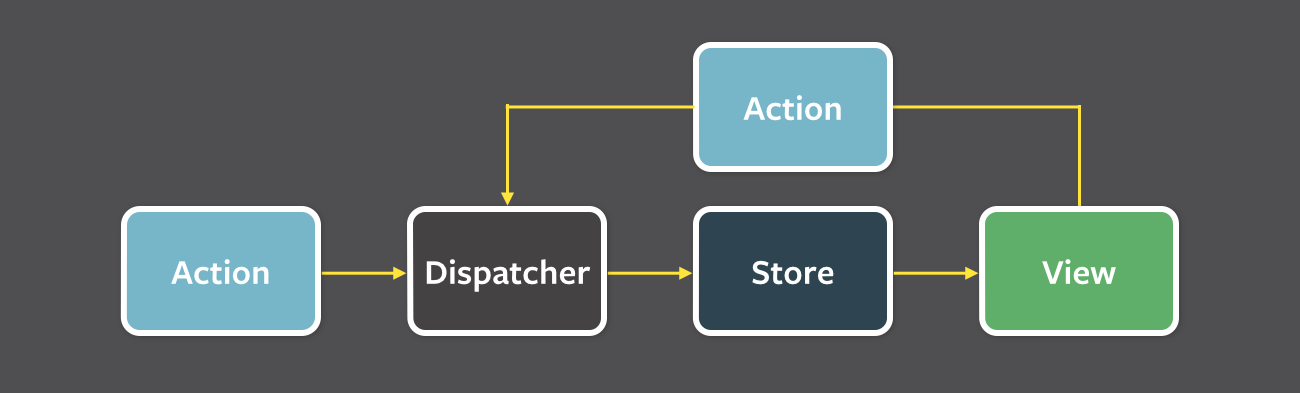
\includegraphics[height=0.25\textwidth]{./images/flux-flow}
	\caption{Datenfluss in der Flux Architektur}
	\label{fig:datenflussFlux}
\end{figure}

Anhand Abbildung \ref{fig:datenflussFlux} wird der unidirektionale Datenfluss deutlich erkennbar:
\begin{enumerate}
	\item Die View schickt eine Aktion an den Dispatcher.
	\item Dieser leitet diese an alle Stores weiter.
	\item Der Store verarbeitet die Daten und informiert die View.
\end{enumerate}
\bigskip
Insgesamt liefert Flux mit diesen Komponenten eine Möglichkeit, einen unidirektionalen Fluss herzustellen und die Verwaltung des Zustands einer Applikation zu vereinfachen.
\subsubsection{Redux}
Bei Redux handelt sich um eine JavaScript Bibliothek (und kein Framework) welche ihre Inspiration aus Flux und Elm bezieht. Sie wurde im Jahre 2015 von Dan Abramov und Andrew Clark ins Leben gerufen.
\cite{reduxIntroduction}
Auch hier nimm der direktionale Datenfluss eine wesentliche Rolle ein.
\\
\\
Die Bibliothek kann als eine vereinfachte Form von Flux verstanden werden, welche gewisse Elemente und Ansätze übernimmt, aber auch streicht bzw. ersetzt. Genau wie Flux existieren die bereits behandelten Actions, welche über wichtige Informationen für die spätere Veränderung des Zustands verfügen. Auch hier können diese ihren Ursprung in einer vom Nutzer getätigten Aktion haben. Wird eine Aktion ausgeführt, so spricht man von einer Versendung einer Aktion. Dieser Versand findet nur dann statt, wenn man die Intention verfolgt, den Zustand zu ändern. Sie gelangt zu einem sogenannten "Reducer". Hier findet sich der erste Grundlegende Unterschied zu Flux.
\\
\\
Ein "Reducer" ist für sich genommen eine einfache Funktion, die bei gleicher Eingabe die immer gleiche Ausgabe erzeugt. Sie ist dabei frei von sogenannten Seiteneffekten und wird als "pure" bezeichnet. Im Falle eines "Reducers" erwartet dieser die vorher erzeugte Aktion und den globalen, derzeitigen Zustand der Anwendung. Sein Aufgabe ist es, aus der Kombination dieser einen neuen Zustand zu generieren. Hierfür wird die Aktion, basierend auf ihrem Typ und eventuellen Inhalt, ausgewertet und der Zustand dementsprechend angepasst. Dabei ist zu beachten, dass keine direkte Manipulation des Zustands möglich ist, stattdessen wird ein komplett neuer Zustand zurückgegeben. Diese Eigenschaft der Unveränderbarkeit wird gemeinhin als "Immutability" erfasst.
\\
\begin{lstlisting}[frame=single, language=Java]
(previousState, action) => newState
\end{lstlisting}
\ \\
Das Verbindungsstück zwischen einer Aktion und dem Reducer bildet der Store. Dieser existiert im Gegensatz zu Flux nur ein einziges Mal (und mit auch der Zustand) und ist für die Verwaltung des Zustands verantwortlich. Er übernimmt zugleich auch die Rolle des Dispatchers, wie er in Flux vorkommt, und verteilt die Akionen an alle Reducer weiter. Der aus dem diesen Prozess hervorgehende, neue Zustand wird im Store hinterlegt. Dieses Ereignis wird ebenfalls seitens der View observiert, welche im Anschluss die nötigen Aktualisierungen an der Ansicht vornimmt.
Am Ende lässt sich der gesamte Fluss wie folgt darstellen:
\\
\begin{lstlisting}[frame=single, language=Java]
View -> Action -> Reducer(s) -> Store -> View
\end{lstlisting}
\bigskip
Neben Redux existieren in der JavaScript Welt noch weitere Bibliotheken, die entweder eine Abwandlungen von Flux darstellen oder aber neue Konzepte implementieren. Jedoch verfolgen dabei alle eine ähnliches Ziel: Ein unidirektionaler Datenfluss und die (zentrierte) Verwaltung des Zustands einer Anwendung.

\subsubsection{Elm}
Bei Flux und Redux handelt es sich jeweils um Bibliotheken die innerhalb einer Anwendung verwendet werden können. Eine weitere Herangehensweise ist die Verankerung solcher Konzepte in der Programmiersprache selbst. Dies findet man z.B. in
der Programmiersprache Elm
\cite{elmIntroduction}
wieder. Elm besitze eine in die Sprache integrierte Architektur die den einfach Namen "The Elm Architecture" 
\cite{theElmArchitecture}
trägt. Eine andere Variante lautet: Model-View-Update. Anhand dessen lassen sich bereits die Kern-Komponenten der Entwurfsmusters erahnen.
\\
\\
\textbf{Model:} Das Model repräsentiert den Zustand der Applikation als eine simple Datenstruktur.
\\
\textbf{View:} Die View ist eine Funktion, welche aus einem Model HTML code generiert. Ebenfalls wie in Flux wird kommt auch hier das Konzept von "pure functions" zum tragen: Die gleiche Eingabe erzeugt die gleich Ausgabe - ohne Ausnahme.
\subsection{Funktionale Programmierung}
Im Verlaufe der Kapitel wurden bereits Begriffe wie eine "reine" Funktion (pure functions) oder die Unveränderlichkeit (Immutibilty) einen Datenstruktur angesprochen. Diese Konzepte zählen zu einem Programmierparadigma, welches in den letzten Jahren auch an Bedeutung in Sprachen wie Java gewonnen hat
\cite{javaFunctionalProgramming}
: Funktionale Programmierung.
\\
\\
In der häufig imperativen, Objektorientierte Programmierung wie sie in Java oder auch C\# anzutreffen ist, machen Klassen und
die Mutation (in möglicher Abhängigkeit von gewissen Konditionen) solcher den Hauptbestandteil des Quellcodes aus. Dabei ist zu beachten, dass die funktionale Programmierung die Objektorientierte nicht zwingenden ausschließt, sondern lediglich in eingeschränkter Form nutzt.
Eine Implementierung in Java welche Beispielweise den Name eines Nutzer Objekts ändert, könnte wie folgt aussehen:
\begin{lstlisting}[frame=single, language=Java]
public User changeUserName(String newUserName, User currentUser){
 if(newUserName != null){
  currentUser.name = newName
		
  System.out.println("Changed user name to: " + newUserName)	
 }
	
 return currentUser
}
\end{lstlisting}

	
%	\newpage
	
%	\section{Model-View-Intent}
\label{sec:model-view-intent}
In diesem Kapitel wird MVI unter die Lupe genommen und genauer beschrieben.

\subsection{Vorausgegangene Architekturmuster}
Hier werden in kurzer Ausführung die bekanntesten Architekturmuster neben Model-View-Intent beschrieben.

\subsubsection{Model-View-Controller}
Mode-View-Controller oder auch MVC ist eines der ältesten Architekturmuster und wurde im Jahre 1979 von Trygve Reenskaug veröffentlicht.
\cite{theModelViewEditorTrygveReenskaug1979, modelsViewsControllersTrygveReenskaug1979}
Es besteht aus drei Komponenten mit folgenden Funktionen:
\begin{itemize}
	\item \textbf{Model}: Es beschreibt den Zustand der Anwendung durch das Festhalten von Daten und aktualisiert informiert die View über Veränderungen. (View)
	\item \textbf{View}: Sie ist für die Darstellung des UI zuständig und aktualisiert sich bei Änderungen im Model.
	\item \textbf{Controller}:  Er kontrolliert die beiden anderen Komponenten und enthält möglicherweise weitere (Business) Logik. Dafür nimmt Ereignisse aus der View bzw. vom Nutzer entgegen und manipuliert daraufhin das Model oder die View direkt. 
\end{itemize}
\begin{figure}[ht]
	\centering
	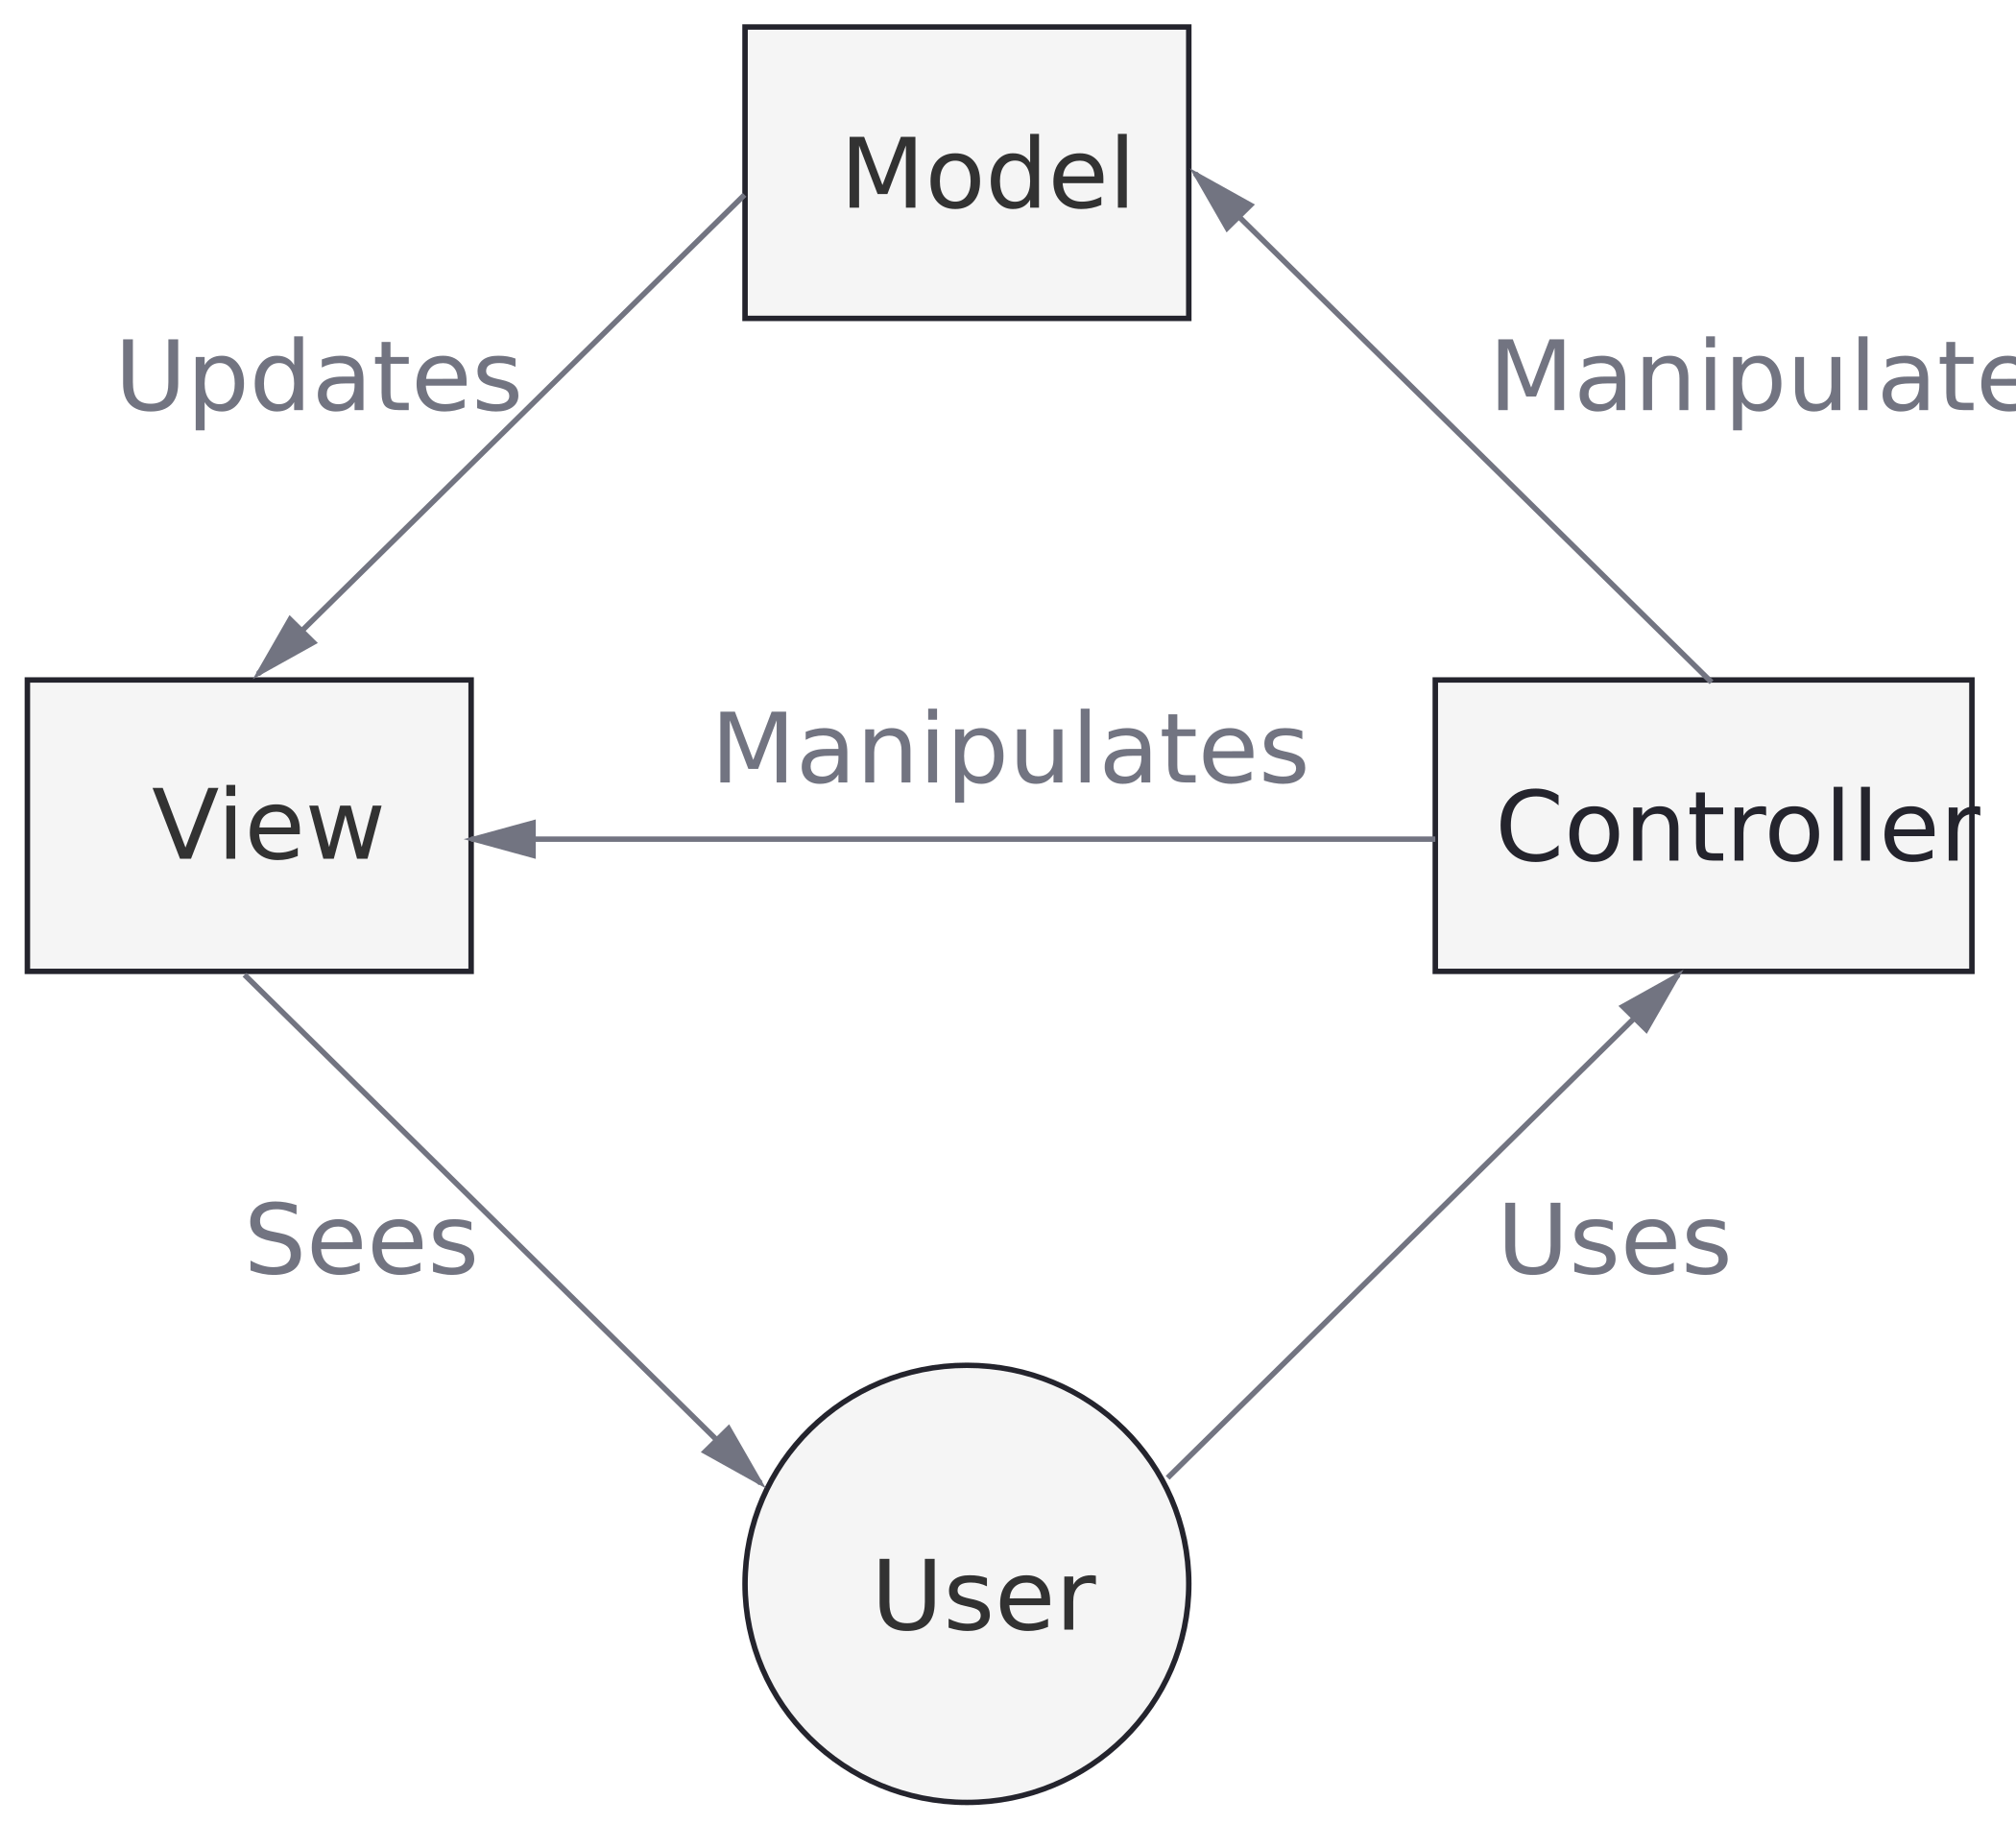
\includegraphics[height=0.5\textwidth]{./images/mvc-diagram.png}
	\caption{Model-View-Controller}
	\label{fig:mvc}
\end{figure}
\clearpage

\subsubsection{Mode-View-Presenter}
Das nächste im Bunde ist Model-View-Presenter (MVP) aus dem Jahre 1996.
\cite{modelViewPresenterTheTaligentMikePotel1996, modelViewPresenterMartinFowler2006}

\subsubsection{Model-View-ViewModel}

\subsection{Historie \& Grundlegendes}
Model-View-Intent (MVI) ist eine weiteres Entfursmuster, welches der Feder von André (Medeiros) Staltz entstammt. Er stellte dieses auf einer Javascript Konferenz im Jahre 2015 vor
\cite{modelViewIntentIntroduction}. Es gehört damit zu den jüngsten seiner Art.
Seine ursprüngliche Anwendung fand es in dem ebenfalls von André Staltz geschaffenen Framework CycleJs, hat seit der Artikelreihe von Hannes Dorfmann in 2016
\cite{modelViewIntentOnAndroidHannesDorfmann2016}
aber auch den Sprung in die Welt von Android vollbracht. MVI bezieht den Großteil seines Design aus den hier bereits vorstellten Ideen und Konzepten. Das erste Ziel ist, ähnlich wie bei MVC, Informationen zwischen zwei Welten zu übersetzten: der des digitalen Bereichs des Computers und des mentalen Modells des Benutzers. Oder anders formuliert: Das Programm muss verstehen, was der Nutzer im Sinn hat.
Der zweite, zentrale Punkt von MVI besteht in der Handhabung des Zustands der Anwendung. Hierfür ist zu klären, was genau der Zustand inne hat.
\\
\\
MVI betrachtet dafür die Interaktion zwischen einem Nutzer und Programm als einen Kreis(lauf). Betätigt der Nutzer bswp. einen Knopf, sein Output, so gestaltet sich dieser als Input für das Programm. Dieses wiederum erzeugt einen Output (z.B. eine Meldung), welcher zum Input des Nutzers wird (hier: lesen).
\begin{figure}[ht]
	\centering
	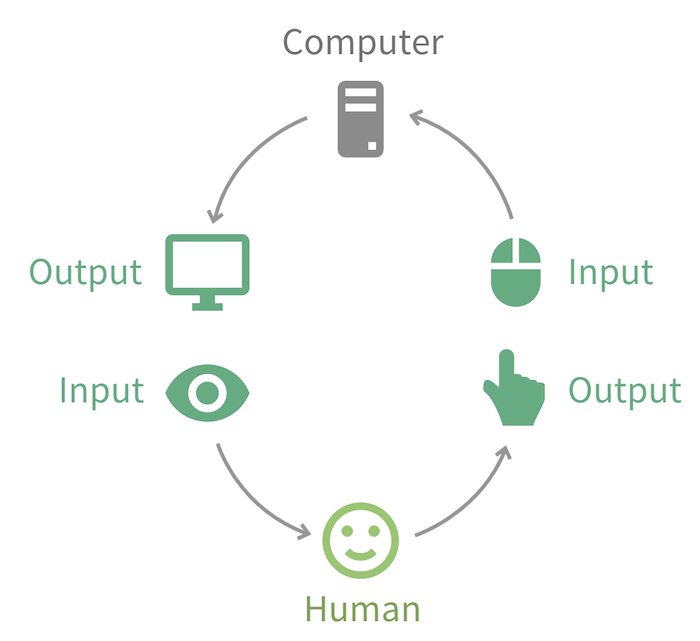
\includegraphics[height=0.5\textwidth]{./images/mvi-cycle}
	\caption{Nutzer und Computer als Input und Output}
	\caption*{Source: https://cycle.js.org/dialogue.html}
	\label{fig:userComputerInputOutput}
\end{figure}
\\
Die Grundprinzipien für den Aufbau der Architektur entspringen dabei dem beschriebenen, originalem Model-View-Controller. Das, was MVC jedoch inkompatibel für die von MVI vorhergesehenen Prozesse macht, ist die Tatsache, das der Controller proaktiv ist. Dies bedeutet, dass der Controller selbstbestimmt über das Model und View verfügen und diese direkt manipulieren kann. Zwangsläufig wissen die jeweiligen Komponenten auch, von welchen Komponenten sie abhängig sind. Oder anders ausgedrückt: Eine Komponente deklariert, welche anderen Komponenten sie beeinflussen, anstatt dass andere Komponenten explizit aktualisiert werden (z.B. das Modell). Dabei wird das Prinzip des unidirektionale Datenfluss verletzt, welches auch in MVI strikt verfolgt wird. 
\\
\\
Um dieses unter anderem zu erreichen, setzt MVI zusätzlich auf Reaktive Programmierung. Für MVI bedeutet reaktiv zu sein, dass jede Komponente ihre Abhängigkeiten beobachtet und auf Veränderungen dieser reagiert. Die drei Komponenten werden durch Observables repräsentiert, wobei der Output jeweils der Input einer anderen Komponente ist.

\subsection{Model, View \& Intent}
Fast noch wichtiger als der reaktive Ansatz ist zu verstehen, wie der Kreislauf in Figur \ref{fig:userComputerInputOutput} 
programmatisch etabliert werden kann. Betrachtet man diesen Kreis etwas genauer, so wird deutlich, dass auf einen Input immer ein Output folgt. Dieses Konzept findet man auch in der Mathematik wieder: Funktionen. Mit diesen lässt sich MVI wie folgt illustrieren:
\\
\\
\textbf{Intent}: Das I in MVI steht für Intent und stellt den Teil da, welches es von den anderen Entwurfsmustern unterscheidet. Das Ziel der Intent-Fuktion ist es, die Absicht des Nutzer im digitalen Kontext des Programms auszudrücken.
Ein Ereignis (oder Event), z.B. die Eingabe eines Buchstaben, kann hier der Input sein.
Der Output dieser Funktion (z.B. ein String) wird zum Input der nächsten:
\\
\\
\textbf{Model}: Die Model-Funktion nimmt das entgegen, was die Intent-Funktion produziert. Ihre Aufgabe liegt in der Verwaltung des Zustands: Sie verfügt über das Model. Sie kann daher durchaus als das zentrale Element in MVI bezeichnet werden. In Anbetracht der Tatsache, dass MVI sich als auf funktionaler Programmierung basierendes Muster versteht, ist das Model unveränderlich. Daraus ergibt sich zwangsläufig, dass für einen Zustandswechsel das Model kopiert und somit ein neues erzeugt werden muss. 
\\
Diese Funktion ist der einziges Teil des Programms, welche eine Zustandsveränderung hervorrufen kann und darf. Zusätzlich ist es der Ort, an dem auf die Business Logik der Anwendung zugegriffen wird.
\\
\\
\textbf{View}: Die View ist die letzte Funktion in der Kette, und ist zuständig für die visuelle Repräsentation des Models.
\newpage
Nimmt man alle drei Funktion zusammen, ergibt sich folgende Kette:
\begin{lstlisting}[caption={funktion}, xleftmargin=.3\textwidth, frame=false, numbers=none]
view(model(intent(input)))
\end{lstlisting}
Um den Sachverhalt zu verdeutlichten, kann dieses Beispiel in Form von pseudo-code herangezogen werden:
\begin{lstlisting}[caption={pseudo mvi implementation}, label={lst:pseudo-mvi}, language=Kotlin]
fun intent(text: String): Event {
	return EnteredTextEvent(text)
}

fun model(event: Event): Model {
	return when(event){
		is EnteredTextEvent -> {
			val newText = event.text.trim() // <-- business logic
			model.copy(text = newText) // <-- immtuable data structure
		}
	}
}

fun view(model: Model){
	textView.text = model.text 	
}

fun main(args : Array<String>) {
	view(model(intent("Hello World")))
}
\end{lstlisting}
Bei dieser Implementierung ist jedoch schnell ersichtlich, das es sich hierbei um keinen Kreis(lauf) handelt. Jede Funktion wird nur einmal aufgerufen. Es fehlt der reaktive Part, der MVI unter anderem ausmacht. Um diesen zu realisieren muss der Beispiel-Code wie folgt abgeändert werden:
\begin{lstlisting}[caption={pseudo mvi implementation},label={lst:pseudo-reactive-mvi},language=Kotlin]
// the obersvable from the textView gets passed as a parameter
fun intent(text: Observabkle<String>): Observable<Event> {
	text.map { text -> EnteredTextEvent(text) }
}

fun model(event:  Observable<Event>): Observable<Model> {
	event.map { event ->
		return when(event){
			is EnteredTextEvent -> {
			val newText = event.text.trim() // <-- business logic
			model.copy(text = newText) // <-- immtuable data structure
		}
	}	
}

fun view(model: Observable<Model>){
	// we subscribe to the model to listen for changes
	model.subscribe { model ->
		textView.text = model.text 	
	}	
}

fun main(args : Array<String>) {

	// this listens to arbitary text changes 
	val textChanges: Observable<String> = textView.changes()

	view(model(intent(textChanges))) 
}
\end{lstlisting}
Ein Punkt der in dieser Implementation noch offen bleibt, ist woher das Model kommt wie es verwaltet wird.

\subsection{Reducer}
Schaut man sich die Model-Funktion in Beispiel \ref{lst:pseudo-reactive-mvi} und ihren Inhalt genau an, so wird ein bestimmtes Muster bzw. ein sich wiederholender Ablauf erkennbar:
\\
\begin{enumerate}
	\item Die Funktion erhält ein Event 
	\item Die Funktion evaluiert das Event
	\item Die Funktion führt basierend auf dem Event (Business) Logik aus
	\item Die Funktion erzeugt ein neues Model
	\item Die Funktion gibt das neue Model zurück
\end{enumerate}
Der einzige Schritt der Fehlt, ist die Bereitstellung des derzeitigen oder des vorherigen Models. Hier kommt eine Komponente ins Spiel, die bereits in Kapitel \ref{subsec:redux} angesprochen wurde: der Reducer.
\subsection{Endlicher Automat}
Wenn der in der Model-Funktion ausgeführte Code eine neues Model hervorbringt, so bleibt der Zustand entweder der Gleiche oder er verändert sich. Unabhängig davon geht der Zustand in den selbigen oder in einen neuen Zustand über: es kommt zu einem sogenannten Zustandsübergang. Aber nicht nur das lässt sich aus dem gezeigten Beispiel ableiten; es sind noch weitere Schlussfolgerungen zulässig:
\\
\begin{itemize}
	\item Es gibt immer einen Anfangszustand bzw. Startzustand
	\item Es gibt eine endliche Anzahl von Zuständen
	\item Es gibt eine beliebe Menge von Endzuständen
	\item Es gibt immer nur einen Zustand, in dem sich die Anwendung befinden kann
\end{itemize}
\bigskip
Die oben genannten Punkte lassen sich anhand eines weiteren Beispiels besser erläutern: Man nehme an, dass sich auf einem Bildschirm ein Textfeld und ein dazugehöriger Knopf befindet. Das Textfeld ist anfänglich leer und der Knopf deaktiviert. Dieser kann nur aktiviert werden, wenn eine Eingabe im Textfeld erfolgt. Hiermit ist der Startzustand des Knopfs "deaktiviert" (z0). Gibt der Nutzer im Textfeld einen Text ein, so wird der Knopf aktiviert. Dieses Ereignis ist der bereits angeführte Zustandsübergang.
Gleichzeitig wird ein Endzustand erreicht (z1) - weitere Eingaben führen zu keinem neuem Zustand.
Die Beschreibungen z1 und z2 dienen hierbei als das Eingabealphabet und zeigen die Menge von potenziellen Ereignissen auf.
\begin{figure}[ht]
	\centering
	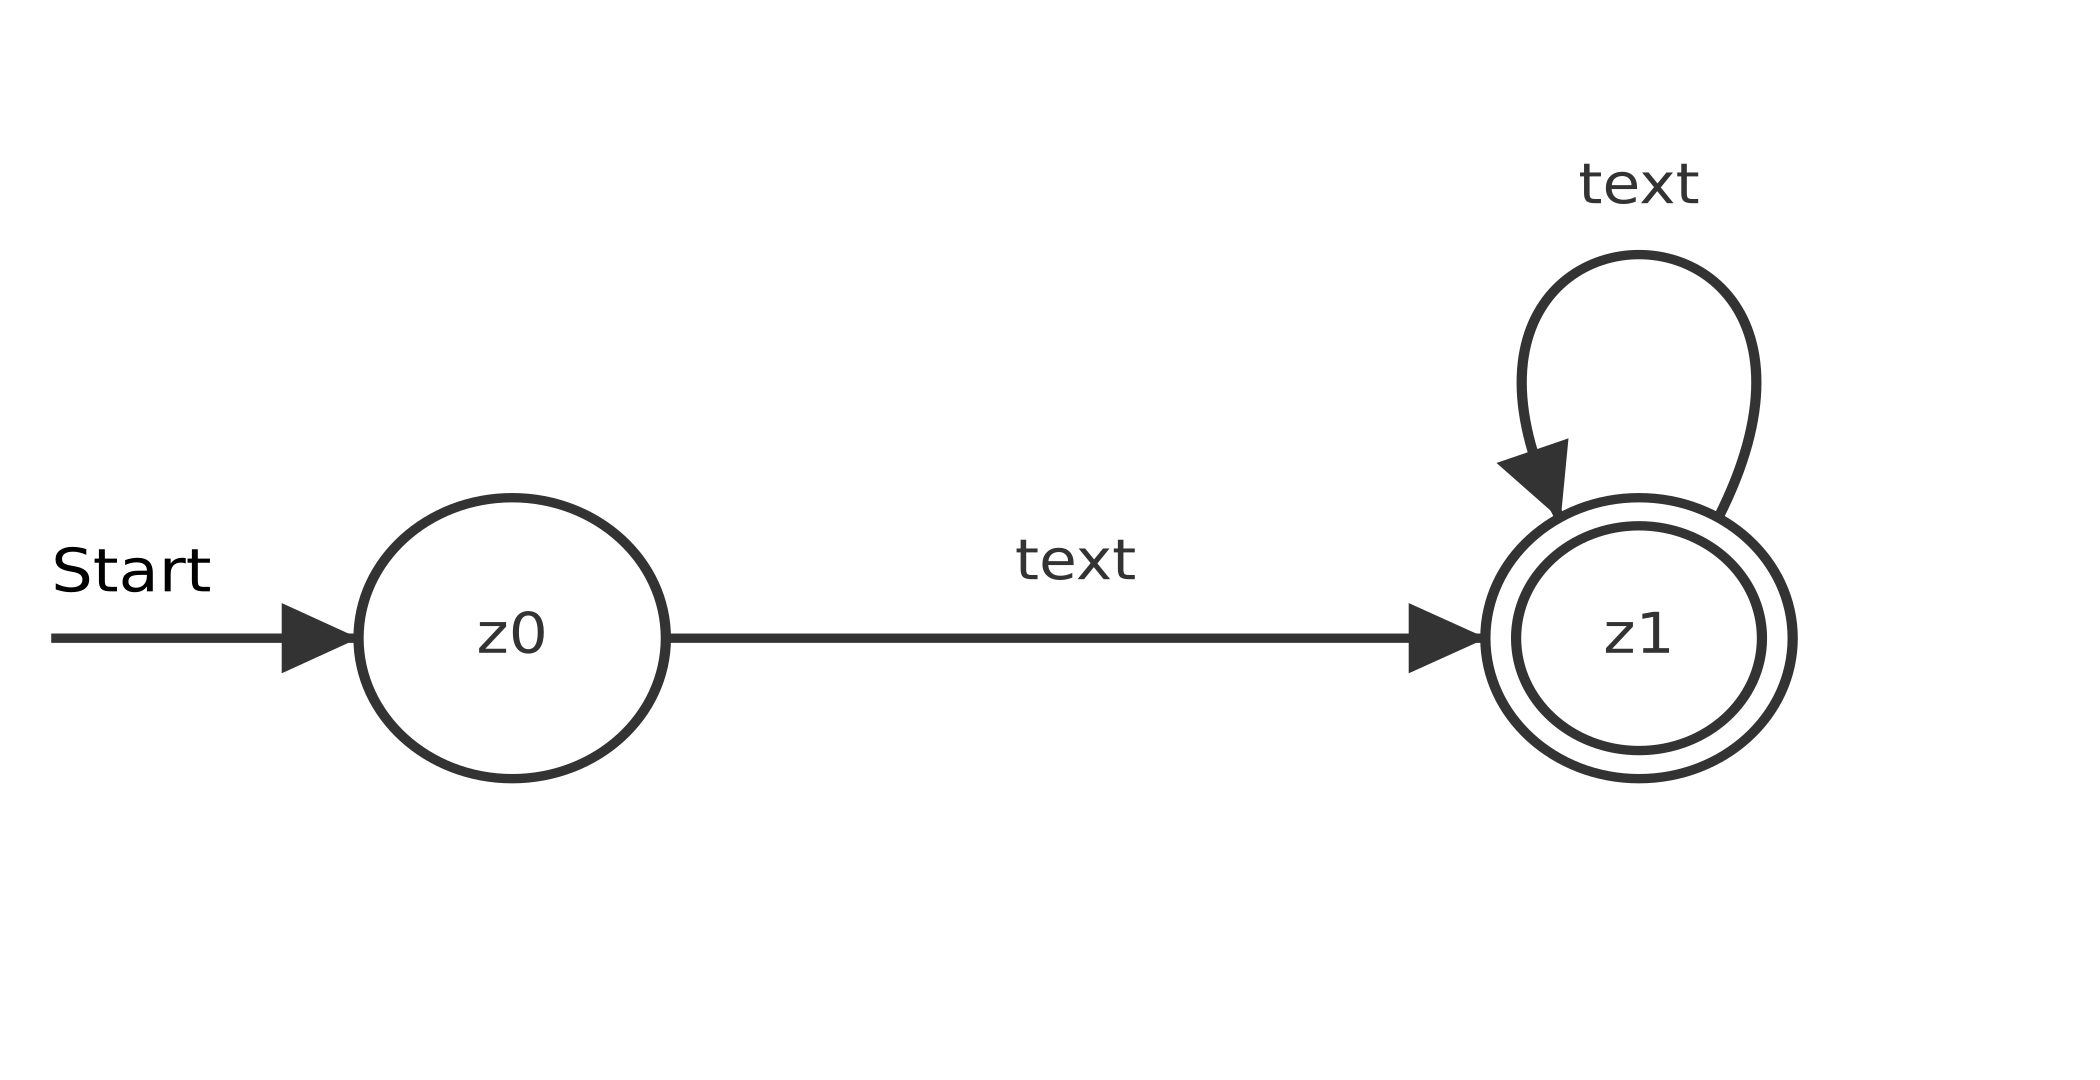
\includegraphics[height=0.35\textwidth]{./images/out}
	\caption{Endlicher Automat}
	\label{fig:endlicherAutomat}
\end{figure}
\\
Dieses Konzept ist in der Informatik bekannt als "Endliche Automaten". Ihr Ziel ist es, ein bestimmtes Verhalten (wie das obige) zu Modellieren und unter anderem visuell in Form von Abbildung
\ref{fig:endlicherAutomat} 
zu präsentieren.
	
%	\newpage
	
%	\section{Anforderungsanalyse}
\label{sec:anforderungsanalyse}

\subsection{Funktionale Anforderungen}
Die Funktionalen Anforderungen dienen dafür, um die genaue Funktionalität und das Verhalten eines Systems zu beschreiben. Es wird behandelt, was das System können soll und muss. Um dies besser abbilden zu können, werden die einzelnen Anforderungen einer Gewichtung unterzogen. Diese Gewichtung lässt sich in Form von "Muss","Soll" und "Kann" Anforderungen ausdrücken. Aufgrund des kleines Rahmens und Zeitfensters dieser Thesis wird sich im diesen Teil ausschließlich auf "Muss"-Anforderungen beschränkt, d.h. jene Funktionalität, welches das Framework erfüllen muss. Für die Übersichtlichkeit werden sämtliche Anforderungen nummeriert und mit dem Kürzel "FA" versehen.
\\
\\
\textbf{[FA01] Identifizieren von "Intents"}
\\
Dem Nutzer des Frameworks muss es möglich sein, die "Intents" seiner Anwendung eindeutig zu markieren.
\\
\\



	
%	\newpage
	
%	\section{Design \& Konzept}
\label{sec:design-und-konzept}
In diesem Kapitel wird sich der Erstellung eines Konzepts für das MVI Framework gewidmet. 

\subsection{Übersicht der Komponenten im Klassendiagramm}
\begin{sidewaysfigure}
		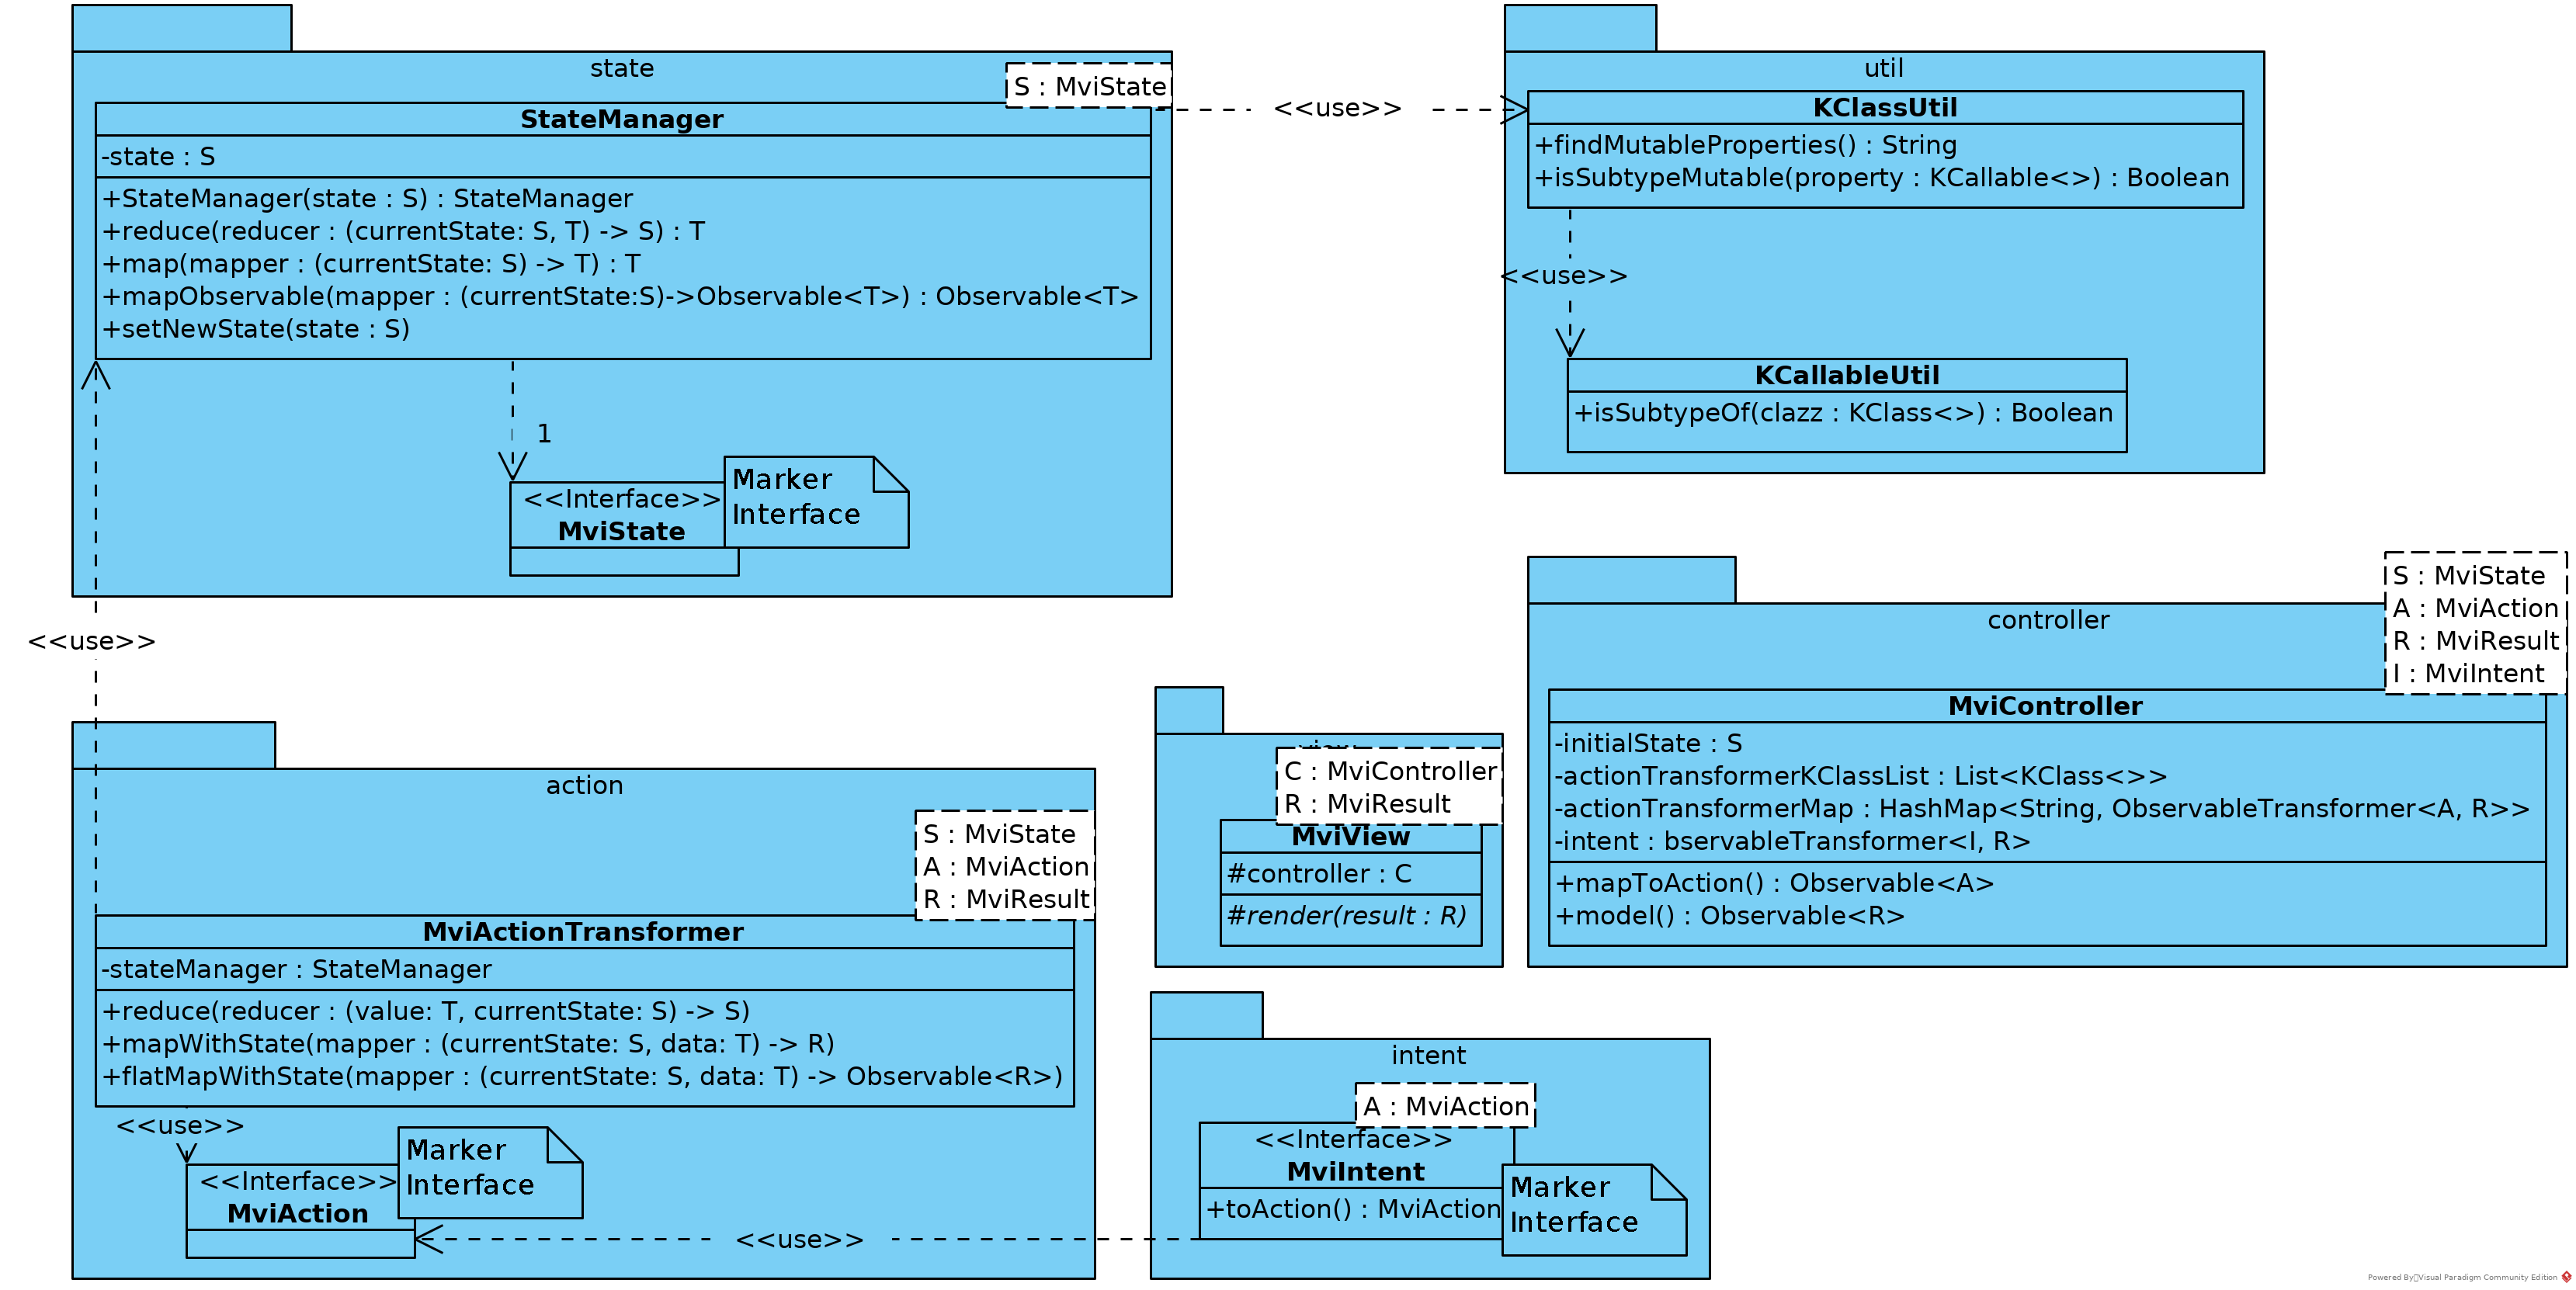
\includegraphics[width=\textwidth]{./images/framework-class-diagram}
		\caption{Komponenten im Klassendiagramm}
\end{sidewaysfigure}
\clearpage
\subsection{Zustand (State) und seine Verwaltung}
\label{subsec:zustand-und-statemanager}
In den Ausführungen von MVI wird der Zustand als eine Anhäufung von Werten betrachtet. Es bildet den Kern von MVI und muss im Normalfall vom Entwickler selbst verwaltet werden. Unter anderem muss garantiert sein, dass ein Zugriff und eine Modifikation des Zustands nur an einer Stelle erfolgen kann. Im Rahmen des Framworks wird eine Komponente genutzt, die diese Aufgaben für den Entwickler übernimmt und den Zustand 'managed': Der 'StateManager'.
\\\\
Dieser erwartet den initialen Zustand, der vom Entwickler an das Framework übergeben wird. Der Zustand wird dabei als generischer Parameter definiert und muss dem Interface 'MviState' entsprechen. Die Variable 'state' selbst ist eine der wenigen, die eine Mutation zulassen muss, wie später deutlich wird.
\\
Nachdem der Zustand überreicht wurde, wird geprüft, inwieweit dieser der Anforderung der Unveränderlichkeit entspricht. Dieser Vorgang wird auf zwei Klassen aufgeteilt: 'KClassUtil' und 'KCallableUtil'. Erstere durchläuft alle Attribute des Zustands und verifiziert, dass keinem dieser ein neuer Wert zugewiesen werden kann. Die letztere schaut, ob auch der Subtyp, z.B eine Liste, nicht direkt modifiziert werden kann. Sollte diese nicht gegeben sein, so wird eine Fehlermeldung ausgegeben und der Prozess gestoppt.
\\\\
Ist dies jedoch erfolgreich, so wartet der 'StateManager' mit Funktionalität auf, welche es ermöglicht einen neuen Zustand zu hinterlegen, sowie mit ihm sicher zu arbeiten. Ein neue Setzung des Wertes wird dabei durch die Kombinationen der Funktionen 'reduce' und 'setNewState' erreicht. 
\\\\
Erstere erwartet eine Funktion als Parameter, 'reducer', welche wiederum den derzeitigen Zustand übergeben bekommt. Diese wird aufgerufen und produziert einen neuen Zustand, der durch 'setNewState' als aktueller Zustand gesetzt wird. Dies geschieht allerdings nur unter der Prämisse, dass sich mindestens ein Wert innerhalb der Datenstruktur verändert hat.
\\
Als Zusatz stellt 'setNewState' sicher, dass es auch bei gleichzeitigen Zugriffen von mehreren 'Threads' zu keiner sogenannten unbeabsichtigten Wettlaufsituation (Race Condition) und damit inkonsistenten Daten kommt.
\\
An dieser Stelle wird erkennbar, weshalb die 'state' Variable zwingend veränderlich sein muss. Wäre diese nicht der Fall, so könnte ihr kein neuer Zustand zugewiesen werden.
\\\\
Die Methode 'map' nimmt genau wie 'reduce' eine Funktionen entgegen, welche den aktuellen Zustand erhält. In dieser kann der Entwickler auf die Attribute des Zustands zurückgreifen, jedoch keine neuen bestimmen.
\\\\
Diese Komponente ist nicht direkt für den Nutzer zugänglich und wird ausschließlich intern im Framework genutzt. Es verhindert, dass der Zustand an einer beliebigen und nicht vorgesehenen Stelle verändert werden kann.

\subsection{Intent, Action und Result}
\label{subsec:intent-action-und-result}
Die im Titel genannten Komponenten dienen der Übermittlung und Beschreibung von Informationen innerhalb des 'Kreislaufs' vom MVI. Diese müssen vom Entwickler selbst gestellt werden, erhalten dabei jedoch Vorgaben vom Framework.
\\\\
So muss zu jedem Intent eine Action existieren. Hierfür wartet das Framework mit dem Interface 'MviIntent' auf, das genanntes erzwingt und die Erfüllung dieser Anforderung sicherstellt. Realisiert wird dies durch die Funktion 'mapToAction', die der Entwickler später implementieren muss und eine 'Action' zurück gibt.  
\\\\
Ähnlich wie auf einen Intent eine Action erfolgt, zieht eine Action ein Result nach sich. Auch das gibt das Framework durch ein Interface namens 'MviAction' vor und muss vom Entwickler angewandt werden. Das Result findet seine Anwendung später in der View und wird ebenfalls mit einem Interface versehen.
\\
\\
Sämtliche der hier aufgeführten Strukturen sollten mit ihrem Namen die vorgesehene Intention signalisieren. Zusätzlich müssen sie in der Lage sein weitere Nutzdaten (Payload) aufzunehmen, die mit ihnen in Zusammenhang stehen und für den weiteren Verlauft essentiell sind.

\subsection{Reaktiver unidirektionaler Datenfluss}
\label{subsec:reaktiver-unidirektionaler-datenfluss}
Für die Konzeptionierung der nächsten Komponenten gilt vorher zu klären, wie der geforderte reaktive unidirektionale Datenfluss in das Framework integriert werden soll. Dabei müssen Daten synchron oder asynchron verarbeitet und die Option zur Nebenläufigkeit (Concurrency) geboten werden. Zu diesem Zweck bedarf es einem Tool, welches das bereits aufgeführte 'Observer' und 'Iterator' Pattern nutzt. In diesem Zusammenhang taucht oft das Objekt 'Observable' auf, das genau diese Anforderungen erfüllt.  

\subsection{Transformer und die Business-Logik}
Ein elementaren Bestandsteil einer Anwendung macht die Businesslogik aus. Sie ist im Falle von MVI allein verantwortlich für das Abändern des Zustands und sollte strikt von anderen Komponenten getrennt sein. Hierfür stellt das Framework den 'ActionTransformer zu Verfügung.
\\\\
Wie der Name vermuten lässt, ist die 'Action' unter anderem ausschlaggebend für die Nutzung der Komponente. Jeder 'Action' wird dabei ein 'MviActionTransformer' zuteil, welche in der ersten der drei generischen Parameter, dem 'A', eingesetzt wird. Dieser Parameter setzt voraus, dass das eingefügte Objekt vom Interface 'MviAction' nutzen macht. Der zweite generische Parameter 'R' sieht ein Objekt vor, dass dem Interface 'MviResutlt' entstammt. Hier wird das zugehörige Result zur angegebenen Action eingefügt. Zuletzt muss der ''MviActionTransformer' wissen, mit welchen Zustand er zu tun haben wird. Dies wird ihm durch den letzten generischen Parameter 'S' mitgeteilt, der als Zuordnung das 'MviState' Interface nutzt. 
\\\\
Der 'MviActionTransformer' ermöglicht die Interaktion mit dem Zustand durch eine Variation an Funktionen. Dafür benötigt er einen 'StateManager' welcher ihm bei seiner Erstellung übergeben werden muss. Die Funktionalität kann dabei - ähnlich wie beim 'StateManger' - in zwei Kategorien unterteilt werden:
\begin{enumerate}
	\item Die, in der ein neuer Zustand erzeugt wird und
	\item die, in der ausschließlich auf die Daten zugegriffen wird
\end{enumerate} 
Zu ersten Kategorie gehört lediglich die 'reduce' Methode, welche auf die gleichnamige Methode im 'StateManager' zugreift. Auch sie bekommt eine Funktion als Parameter, jedoch mit dem Unterschied, dass diese zusätzlich den derzeitigen Wert in Bearbeitung enthält. Dies kann beispielsweise ein Item sein, dass von einem Intent an die Action weitergegeben wurde. Auf Basis dieser zwei Werte kann der Entwickler einen neuen Zustand bestimmen, welcher intern über den 'StateManager' gesetzt wird. Diese Operation findet auf der in Abschnitt
\ref{subsec:reaktive-programmierung}
präsentierten 'Observable' Klasse statt und legt diese auch mit 'T' als Rückgabewert fest.
\\\\
In die zweite Kategorie fallen die Methoden 'mapWithState' und 'flatMapWithState', die beide die gleiche Funktion wie sie auch bei 'reduce' verwendet wird erhalten. Ihnen ist es nicht gestattet eine neuen Zustand herzustellen, sie können lediglich mit ihm arbeiten. Die 'flatMapWithState' Methode grenzt sich dadurch ab, das sie erlaubt andere asynchrone Funktionalität auszuführen, die ebenfalls einen Wert vom Typ 'Observable' zurückgibt und dabei Seiteneffekte berücksichtigt.
\\
Alle hier aufgezählten Methoden operieren auf den anfangs genannten generischen Parametern. 
\\\\
Somit ist im Quellcode klar ersichtlich, inwieweit eine Abänderung der Zustands gewollt ist und wann dieser lediglich mitsamt seiner Daten für den weiteren Verlauf benötigt wird. Hinzu kommt hier auch die automatische Handhabung von Seiteneffekten und asynchroner Funktionalität. Dies garantiert, dass der Zustand keine unabsichtliche Modifikation erfährt und zu jedem Zeitpunkt nur einer auf ihn zugreifen kann.

\subsection{Controller als Bindeglied}
Der Controller vereint die bisher beschriebenen Komponenten und 'kontrolliert' bzw. koordiniert anhand dieser den Aufruf der Business-Logik. Er stellt das Bindeglied zwischen der View, einer 'Action' und dem dazugehörigen 'ActionTransormer' dar und sorgt für den Aufruf von ebendiesem. 
\\\\
Dafür muss er über die vom Entwickler angedachte Form des Zustands, Intents, Action und Result informiert werden. Dies geschieht wie bei den vorherigen Komponenten durch die Angabe mehrerer generischer Parameter. Überdies erhält der Controller für seine Konstruktion den initialen Zustand und eine Liste von Namen der zugehörigen 'MviActionTransformer' vom Entwickler.
\\\\
In der initialen Phase verifiziert der 'Controller', dass alle 'ActionTransformer' von der hinterlegten 'Action' und dem 'Result' abstammen um späteren Konflikten vorzubeugen. Anschließend wird der 'StateMananger' mit dem überlieferten Zustand instanziiert. Im letzten Schritt erzeugt der 'Controller' alle 'ActionTransformer' die jeweils einen 'StateManager' zugewiesen bekommen und speichert diese in Form von Schlüssel (Name des Transformers) und dazugehörigem 'ActionTransformer' in dem Attribut 'actionTransformerMap' ab.
\\\\
Im Controller selbst existieren zusätzlich zwei Funktionen und eine Variable, von denen nur letztere von außen zugänglich ist: 'intent'. Sie stellt die in MVI beschriebene Intent-Funktion dar und dient als Einstieg in den unidirektionalen Kreislauf. Wird sie aufgerufen so führt sie die interne 'mapToAction' Methode aus, die mittels der im 'MviIntent' Interface definierten 'toAction' Methode, den 'Intent' in eine 'Action' umwandelt.
\\\\
Die zweite und zugleich auch letzte Funktion ist die 'model' Methode. Sie nimmt die 'Action', ermittelt ihren Klassennamen und entnimmt auf Grundlage dessen den entsprechenden 'ActionTransformer' aus der 'actionTransformerMap'. Die dort enthaltende Business Logik wird dann ausgeführt und das 'Result ', verpackt in einem 'Observable', nach 'oben' durchgereicht.
\subsection{View}
Die 'View' stellt den obersten Teil des Frameworks dar und besitzt im Kern zwei Eigenschaften: Sie reicht die 'Intents' an ihren 'Controller' weiter und verarbeitet das von ihm erhaltene 'Result'. Für beide werden erneut generische Parameter definiert. Einmal einer welcher aussagt, dass das eingefügte Objekt vom 'MviController' abstammen und ein zweiter, der dem 'MviResult' Interface entsprechen muss.
\\\\
Hierfür etabliert das Framework die 'MviView' Klasse, von der die 'View' abstammen muss. Sie stellt die oben geschilderten Anforderungen sicher, indem sie den Entwickler zwingt, ein Attribut zu hinterlegen und eine Funktionen zu implementieren. Bei ersterem handelt es sich um das Objekt, dass der Entwickler als 'MviController' ersonnen hat, bei letzterem um eine Methode, die ein 'Result' als Parameter erwartet. In dieser soll vom Entwickler die Logik stehen, welche für das Aktualisieren des User Interface (UI) zuständig ist. 

\subsection{Anleitung zur korrekten Nutzung}
Um die Handhabung des Frameworks und die für den Entwickler vorgesehenen Komponenten besser nachzuvollziehen, wird im folgenden eine kurze Schritt für Schritt Anleitung dargelegt:
\begin{enumerate}
	\item Anlegen der Klasse für den Zustand im Verbund mit 'MviState'
	\item Anlegen sämtlicher Actions im Verbund mit 'MviAction
	\item Anlegen sämtlicher Intents im Verbund mit 'MviIntent' und obigen 'Actions'
	\item Anlegen sämtlicher Results im Verbund mit 'MviResult'
	\item Implementierung der Business Logik auf Basis der 'MviActionTransformer' Klasse
	\item Implementierung des Controllers auf Basis der 'MviController' Klasse
	\item Implementierung der View auf Basis der 'MviView' Klasse
\end{enumerate}
\bigskip
Soll eine weitere 'Action' hinzugefügt werden, so muss diese lediglich in der jeweiligen Klasse mit ihrem 'Result' hinterlegt werden. Danach erfolgt die Erstellung des dazugehörigen 'MviActionTransformer' samt Business Logik. Zuletzt wird dieser der 'KClass<*>' Liste die der 'MviController' erwartet beigefügt.
\\\\
Insgesamt ist der anfängliche Aufwand wie oft üblich etwas höher, beschränkt sich danach aber für jeden Zusatz auf das zuletzt beschriebene Vorgehen.
	
%	\newpage
	
%	\section{Prototypische Implementierung}
\label{sec:prototypische-implementierungt}
In diesem Kapitel findet auf Basis des zuvor angefertigten Konzepts eine prototypische Implementierung statt. Zu Beginn wird dabei auf Entscheidungen eingegangen, die globalen Einfluss auf die Umsetzungen haben.

\subsection{Grundlegende Entscheidungen}
In diesem Teil werden Themen besprochen, die Auswirkungen auf den weiteren Verlauf der Implementation haben.

\subsubsection{Android als Plattform}
Das Framework richtet sich ausschließlich an Entwickler die Applikationen für die Plattform Android entwickeln. Es ist damit nicht kompatibel zu iOS, dem Web oder serverseitigen Anwendungen. Die Spezialisierung lässt es jedoch zu, besser auf mögliche Eigenheiten der Plattform einzugehen. Ein weiterer Grund für diese Entscheidung stellt die Tatsache dar, dass MVI seinen Anfang in der Entwicklung von Webseiten fand und erst später seinen Einzug in Android erhielt.

\subsubsection{Kotlin als Programmiersprache}
Die Applikationen in Android und das Android-SDK selbst sind bis vor wenigen Jahren fast ausschließlich in der Sprache Java entwickelt wurden. Seit der Google I/0 2017 gehört jedoch eine weitere Sprache zu den offiziell unterstützten:  Kotlin. Sie wird von dem Unternehmen Jetbrains
\footnote{https://www.jetbrains.com/}
entwickelt, die untere anderem die Entwicklungsumgebung Intellij für Java produzieren. Dieses bildet auch die Grundlage für Android Studio.
Kotlin hat in den letzten Jahren an Bodenhaftung gewonnen und findet auch intern bei Google Verwendung.
\\
Die Sprache wird als statisch typisierte, objektorientierte Programmiersprache bezeichnet und verfügt über eine hohe Interoperabilität zu Java. Dies bedeutet, dass innerhalb eines in Java geschriebenen Programms ohne viel Aufwand Kotlin genutzt werden kann. Dies ist ein wichtiger Faktor für die immer weiter ansteigende Beliebtheit, da es eine einfache Integration für bisherige Projekte gestattet. 
Kotlin bringt eine verbesserte Syntax mit und macht beispielsweise die Verwendung von »null« explizit.
Zu den Verbesserungen gehören dabei auch:
\\
\begin{itemize}
	\item Ableitung von Typen
	\item Alles ist eine Expression 
	\item Funktionen sind »First-Class-Objekte« und bilden eine funktionale Grundlage
	\item Datenklassen machen den Umgang mit unveränderliche Datenstrukturen einfach
	\item Erweiterungsfunktionen
	\item Kovarianz und Kontravarianz werden explizit anwendet
	\item Standardwerte für Parameter
\end{itemize}
\bigskip
\begin{lstlisting}[caption={Kotlin Beispiel}, label={lst:kotlin-beispiel}, language=Kotlin]
data class Example(
  privat val defaultMessage: String = "Hello World"
  privat val maybeNull: String? = null
){
  
  // Expression
  fun isHelloWorld() = when(message){
    "Hello World" -> true
    else -> false
  }
  
  // "?" findet bei null verwendung
  fun printIfNotNull() {
    maybeNull?.run { 
    	print(this)
    }
  }
}

// Erweiterungsfunktion und Funktion als Parameter
fun Exampaple.extensionFunction(function: () -> String) { 
	val message = function()
	println(message)
}

// kein new Schlüsselwort nötig
// keine Semikolon nötig
val example = Example()

// copy wird automatisch generiert bei einer "data" Klasse
val newExample = example.copy(defaultMessage = "New Message")

// ist der letzte Parameter eine Funktion, so kann auf Klammern 
// verzichtet werden
newExample.extensionFunction { "Hello" }
\end{lstlisting}
\bigskip
Insgesamt is anhand Listing
\ref{lst:kotlin-beispiel}
zu erkennen, das Kotlin eine deutlich prägnantere und schlankere Syntax besitzt. Sie vermeidet damit einen großen Teil des mit Java verbundenen »Boilerplate-Codes« und kann für eine höheren Grad an Produktivität sorgen. Besonders der Umgang von Null als Teil des Typsystems kann vor der berühmten »Nullpointer-Exception« retten. Des weiteren besteht ein größerer Fokus auf dem Einsatz von Konzepten aus der funktionalen Programmierung, welche durch Erweiterungsfunktionen für bspw.. Listen zum Einsatz kommen.

\subsection{Funktionale reaktive Programmierung mit RxJava und RxKotlin}
Die Implementierung des Obervers und Iterator Patterns mit dazugehörigen Operatoren, die Einhaltung von funktionalen Paradigmen und die Berücksichtigung von asynchroner als auch paralleler Ausführung von Funktionalität (und deren Synchronisierung) ist eine äußerst komplexe Herausforderung, die viel Erfahrung und Zeit erfordert. Deshalb wird in diesem Fall auf eine bereits bestehende Implementierung zurückgegriffen, die in der Android Entwicklung oft zur Anwendung kommt: RxJava.
\\\\
Diese Bibliothek ist eine Implementierung der »Reactive Extension« API, welche für viele Plattformen und Programmiersprachen verfügbar ist. Sie hat ihrem Ursprung in ».NET/C\#« aus dem Hause Microsoft. Sie arbeitet genau wie die Java Stream API auf der Basis von Datenströmen und stellt dafür ein Fülle an Operatoren zur Verfügung.
\\\\
Zusätzlich zu »RxJava« existiert eine DSL (»Domain Specific Language«) die Kotlin agnostisch ist: »RxKotlin«.
Anhand Listing
\ref{lst:rx-beispiel}
soll der Umgang mit dieser Bibliothek in einem für den weiteren Verlaufen relevanten Umfang dargelegt werden.
\begin{lstlisting}[caption={RxJava/Kotlin Beispiel}, label={lst:rx-beispiel}, language=Kotlin]
// Erstellung eines Observables
val observable = Observable.just("Hello")

observavble
	.map { text: String ->
		text + "World"
	}.subscribe(::println)
\end{lstlisting}

\subsection{Zustand (State) und der StateManager}
Ähnlich wie bei Redux nimmt das Model in MVI und somit der Zustand die zentral Rolle innerhalb der Anwendung ein. Es diktiert das User Interface (UI) und hat wesentlichen Einfluss auf die ausführende Business-Logik.
\\
\\
Für die Repräsentation des Models gibt MVI vor, das dieses unveränderlich sein muss. Dies wiederum hat zur Folge, dass für jede Zustandsüberführung ein neues Model auf Basis des alten bzw. derzeitigen erzeugt werden muss. Hierfür wird der Zustand kopiert und während diesem optionalem Vorgang mit neuen Werten versehen. 
\\
\\
Für dieses Szenario stellt Kotlin eine Struktur zur Verfügung, welche den Prozess stark vereinfacht: Die »data« Klasse. Sie generiert unterschiedliche Methoden welche dem Nutzer ohne weiteres Zutun zur Verfügung stehen. Darunter befindet sich unter anderem die Methode »copy«. Wie der Name vermuten lässt, erzeugt sie eine Kopie der Klasse. Dabei können der Methode die Parameter übergeben werden, welche der Konstruktor der Klasse inne hat. Dies macht es möglich einzelne Attribute neu zu besetzten und bei den übrigen den derzeitigen Wert beizubehalten. Wie Listing
\ref{lst:data-class}
aufzeigt, gestaltet das den Umgang mit unveränderlichen Klassen verhältnismäßig einfach.
\begin{lstlisting}[caption={data class}, label={lst:data-class}, language=Kotlin]

data class MyClass(val text: String, val anotherText: String)

val myClass = MyClass("text", "anotherText")

// "text" wird verändert, "anotherText" nicht
val newMyClass = myClass.copy(text = "newText")
\end{lstlisting}
\bigskip
Eine Problematik die herbei jedoch besteht ist, dass bei der »data« Klasse unveränderliche Attribute (= val) keine Pflicht darstellen. Somit wäre es dem Entwickler ohne weiteres Möglich, die Instanz direkt zu modifizieren, ohne ein neue zu erzeugen müssen. Um das zu verhindern gilt es sicherzustellen, dass das vom Entwickler angedachte Model den Anforderungen der Unveränderlichkeit entspricht. Für diesen Zweck kann aus zwei »Werkzeugen« gewählt werden: Der Reflexion (oder Introspektion) und dem Generieren von Code.  
\subsubsection{Reflexion (Introspektion)}
Bei dieser Variante ist es dem ausführenden Programm erlaubt seine eigene Struktur - zur Laufzeit - zu analysieren oder auch zu verändern (und Sichtbarkeitseinschränkungen zu umgehen). Es gestattet einem, Informationen über Klassen dynamisch auszulesen. Das beinhaltet Zugriffsmodifikatoren, Variablen, Konstruktoren, Methoden, Annotationen (= Metadaten) usw. Reflexion hat dabei vielfältige Anwendungszwecke:
\begin{enumerate}
	\item Debugger
	\item Interpreter
	\item Objektserialisierung
	\item Dynamisches Laden von Code/ Erzeugen von Objekten (z.B. Spring @Autowired)
	\item Java Beans
\end{enumerate}
\bigskip
In Kotlin muss beachtet werden, dass zwei Schnittstellen für den Einstieg in die Reflexion existieren. Einmal die Standard Schnittstelle für Java, und einmal jene für Kotlin. Erstere erlaubt die Arbeit mit allen Java Konstrukten und zweitere die, die Kotlin exklusiv sind. Für jede Klasse existiert zur Laufzeit ein Objekt des Typs »Class<T>« oder KClass<T>. T ist dabei der Typ der zu untersuchenden Klasse.
\\
\\
Für den Zugriff auf die Java Reflexion muss auf die ».java« Endung zurückgegriffen werden, wie folgendes Beispiel verdeutlicht:
\begin{lstlisting}[caption={Java Reflexion}, label={lst:data-class}, language=Kotlin]

val myClass: Class<MyClass> = MyClass::class.java

// gibt Methoden wie "toString" aus
myClass.methods.forEach(::println)
\end{lstlisting}
\bigskip
In Kotlin wird über den »double-colon« Operator auf die Reflexion zugegriffen:
\begin{lstlisting}[caption={Kotlin Reflexion}, label={lst:data-class}, language=Kotlin]

val myClass: KClass<MyClass> = MyClass::class

// gibt den Namen der Klasse aus
println(myClass.qualifiedName)

// "false", da "text" nicht Konstant ist
println(myClass::text.isConst)
\end{lstlisting}
\bigskip
Eine weiterer, durchweg interessanter Ansatz ist die Arbeit mit sogenannten Metadaten. Sie stellen Information über Informationen dar. Ein häufiger Anwendungsfall ist die Arbeit mit Annotationen, welche mit »@« eingeleitet werden. So wird mit der »override« Annotation dem Compiler in Java mitgeteilt, dass diese Methode überschrieben wurde:
\begin{lstlisting}[caption={Override Annotation}, label={lst:data-class}, language=Kotlin]

class MyClassJava {

@Override
public String toString() {...}
}

class MyClassKotlin {

// Hier ist "override" teil der Deklaration
override fun toString() {...}
\end{lstlisting}
\bigskip
Anhand der Beispiele lässt sich erahnen, dass Reflexion beträchtlichen Einfluss auf die Anwendung haben kann und viele Türen öffnet. Wie üblich ergeben sich dabei gewisse Vor- und Nachteile:
\\
\\
\textbf{Vorteile:}
\begin{itemize}
	\item Analysieren und modifizieren von Klassen zur Laufzeit
	\item Erweiterbarkeit durch die Nutzung von Annotationen 
\end{itemize}
\textbf{Nachteile:}
\begin{itemize}
	\item Der Zugriff auf private APIs kann ein Sicherheitsrisiko darstellen
	\item Es kann nicht überprüft werden, inwieweit ein korrekter Datentyp vorliegt
	\item Es kann die Ausführungsgeschwindigkeit negativ beeinflussen, da die JVM Optimierungen nicht durchführen kann 
\end{itemize}
Angesichts dieser Auflistung lässt sich festhalten, dass der Gebrauch von Reflexion auf das notwendige Maß beschränkt werden sollte, da es grundlegende Prinzipien der typisierten Programmierung verletzt.

\subsubsection{Code Generation}
Ein andere Methodik besteht in der Generierung von Code. Hierbei wird ein Programm geschrieben, welches wiederum ein anderes Programm erzeugt. Ein Grund kann z.B. ein repetitiver Prozess sein, der somit automatisiert werden kann. Eine beliebtes Verfahren ist das Produzieren von Klassen basierend auf ».json« Dateien.
\\
\\
Mithilfe der Bibliothek "KotlinPoet" kann durch folgenden Code...
\begin{lstlisting}[caption={Code zum erezugen einer Funktion}, label={lst:data-class}, language=Kotlin]
FunSpec.builder("add")
	.addParameter("a", Int::class)
	.addParameter(ParameterSpec.builder("b", Int::class)
	.defaultValue("%L", 0)
	.build())
	.addStatement("print(\"a + b = ${ a + b }\")")
	.build()
\end{lstlisting}
\bigskip
folgender Code erzeugt werden:
\begin{lstlisting}[caption={Erzeugte Funktionen}, label={lst:data-class}, language=Kotlin]
fun add(a: Int, b: Int = 0) {
	print("a + b = ${ a + b }")
}
\end{lstlisting}
welcher in einer ».kt« abgelegt wird. Auf diese Funktion haben sämtliche Klassen zugriff.
\subsubsection{Überprüfung durch Reflexion}
Um die Wartung von generiertem Code, den Aufwand der Implementierung und damit einhergehenden Zeitaufwand zu umgehen, fällt die Entscheidung auf Reflexion. 
\\\\
Im ersten Schritt muss verifiziert werden, dass es sich bei der Klasse für den Zustand um eine »data« Klasse handelt. Hierfür bietet die Kotlin Reflexion API ein Attribut:
\begin{lstlisting}[caption={Kotlin »isData« Attribut}, label={lst:data-class}, language=Kotlin]
data class DataClass

println(DataClass()::class.isData) // true
\end{lstlisting}
\bigskip
Sollte diese Auswertung negativ ausfallen, so wird eine »IllegalStateException« geworfen und dem Entwickler mitteilt, dass ohne eine »data« Klasse nicht fortgefahren werden kann.
\\\\ 
Ist die Überprüfung jedoch erfolgreich, so muss im weiteren Vorgehen die einzelnen Attribute der Klasse auf ihre Unveränderlichkeit überprüft werden. Um dies zu erreichen, kann auf Basis folgender Schritte eine Implementierung stattfinden:
\begin{enumerate}[label*=\arabic*.]
	\item Liste sämtlicher Attribute der zu prüfenden Klasse erstellen
	\item Filtern von nicht benötigten Attributen
	\item In einer »Schleife« 
	\begin{enumerate}[label*=\arabic*.]
		\item Prüfen, inwiefern das Attribut »var« als Zugriffsmodifikator verwendet wird
			\subitem Bei Gebrauch zusätzlich den Typen auf Unveränderlichkeit prüfen
		\item Typen auf Unveränderlichkeit prüfen
		\item Eine Fehlernachricht generieren, mit den veränderlichen Attributsnamen
	\end{enumerate}
	\item Eine Fehlernachricht mit allen veränderlichen Attributen oder einen leeren Text zurückgeben
\end{enumerate}
Die Funktion zu Überprüfung wird dabei als Erweiterungsfunktion auf der Klasse »KClass«, Kotlins Klasse für Metadaten, realisiert. Diese besitzt einen generischen Parameter und erwartet einen Typ. Damit sie für alle Typen gültig ist, wird als Typ das Sternzeichen hinterlegt. Es handelt sich dabei um einen sogenannte »Wildcard« und sagt aus, das beliebige Typen möglich sind.
\\\\
Innerhalb der Erweiterungsfunktion erfolgt der Zugriff auf die Liste aller Attribute der Klasse (Listing
\ref{lst:erweiterungsfunktion-kclass-01}).
\begin{lstlisting}[caption={Erweiterungsfunktion »KClass« mit Liste aller Attribute}, label={lst:erweiterungsfunktion-kclass-01}, language=Kotlin]
internal fun KClass<*>.findMutableProperties(): String =
	members // Liste mit allen Attributen
	// ...
\end{lstlisting}
\bigskip
Zu beachten ist dabei, dass bei der »data« Klasse für jedes Attribut ein zusätzliches generiert wird, welches mit dem Wort »component« beginnt und am Ende eine Zahl von eins bis n (= Anzahl der Attribute) stehen hat. Durch dieses kann das Verfahren der destrukturierenden Zuweisung angewandt werden. Hierbei können aus dem Objekt Daten extrahiert und in (mehreren) Variablen abgelegt werden. Dies ist z.B. nützlich, wenn eine Funktion zwei Werte zurückgeben, oder eine »Map« mit Schlüssel und zugehörigem Wert gleichzeitig durchlaufen werden soll. Listing
\ref{lst:destrukturierende-zuweisung}
zeigt beide Anwendungsfälle.
\begin{lstlisting}[caption={Destrukturierende Zuweisung}, label={lst:destrukturierende-zuweisung}, language=Kotlin]
data class Person(
	val forename: String,
	val surname: String
)

fun fetchPerson() = Person("forename", "surname")

val (forename, surname) = fetchPerson()

for ((key, value) in map) {
	// .... 
}
\end{lstlisting}
Damit keine doppelte Überprüfung eines Attributs durch die »componentN« Variable erfolgt, müssen diese vorher aus der Liste entfernt werden. Zu diesem Zweck wird eine Filter Methode angewandt, die den Namen jeden Attributs daraufhin untersucht. Entspricht es dem Suchmuster, so wird es - entsprechend Listing 
\ref{lst:filtern}
- aus der Liste gelöscht.
\begin{lstlisting}[caption={Filtern}, label={lst:filtern}, language=Kotlin] 
members.filter { property -> 
	property.name.startsWith("component").not() 
}
\end{lstlisting}
\bigskip
im weiteren Verlauf herausgefiltert. 
\\\\
Daraufhin soll geschaut werden, inwiefern eine Variable vorliegt, welcher ein neuer Wert zugewiesen werden kann. Dies ist der Fall, wenn dem Namen der Variable das Schlüsselwort »var« vorausgeht. Mit der Reflexion API wird dies über die »KMutableProperty<*>« Klasse signalisiert. Diesem schließt sich die Überprüfung auf Unveränderlichkeit des Subtyps an. Darunter fällt beispielsweise eine »MutableList« in Kotlin, welcher Elemente direkt hinzugefügt oder entfernt werden können. Für jeden Fund wird eine Fehlermeldung erzeugt, die angibt welches Attribut betroffen ist. Diese wird an die vorherige Fehlermeldung angeheftet und zum Schluss im Gesamten als »String« zurückgegeben.
Hierfür muss die Liste in einer Schleife durchlaufen werden und in jedem Durchlauf die bisherigen Fehlermeldung in Form eines »String« bereitstellen. 
\\\\
Eine Möglichkeit wäre die Standard »for« Schleife in Kombinationen mit einer veränderlichen String Variable. Dies ist jedoch nicht dem Ziel der Fokussierung auf funktionale Konzepte vereinbar und ist daher keine Option. Zur Hilfe kommt die »fold« Methode: Sie summiert den Wert, welcher mit einem Anfangswert festgelegt wird, und führt auf Basis einer Funkion und dem letzten Wert eine Operationen aus, die immer als Rückgabewert den Typ des Anfangswert hat. Zuletzt gibt sie den summierten Wert zurück.
\\\\
In diesem Fall ist der anfängliche Wert einer leerer »String«, an den Fehlermeldungen angehängt werden können. Dabei wird nicht der String selbst verändert, sonder es wird eine Kopie erzeugt. »String« ist von Haus aus »Unveränderlich«. Darauf folgt die Funktionen, die die oben aufgeführten Schritte umsetzt. Ihr erster Parameter ist »errorMessage« und entspricht dem Typ des Anfangswert (hier: String). Der zweite, »property«, ist vom Typ »KCallable<*>« und bezeichnet einen Wert aus der Liste »members«. Es ist ein Attribut des Zustands das überprüft werden soll.
\\\\
Im Funktionskörper befindet sich eine »when« Expression die ist zu erst abfragt, inwiefern es sich um eine »KMutableProperty« Klasse handelt. Trifft dies zum, so wird eine temporäre Fehlerbeschreibung erstellt und mitsamt des Attributs an die nächste Funktion weitergereicht. Diese schaut mittels »property.isSubtypeOf(MutableList::class)« bspw. ob es sich um eine »MutableList« handelt. »isSubtypeOf« entstammt nach Listing
\ref{lst:kcallableutil}
der »KCallableUtil« Klasse und nimmt die Überprüfung des Subtypen vor.
\begin{lstlisting}[caption={KCallableUti}, label={lst:kcallableutil}, language=Kotlin]
internal fun KCallable<*>.isSubtypeOf(clazz: KClass<*>)
	: Boolean = returnType.isSubtypeOf(clazz.starProjectedType)
\end{lstlisting}
\bigskip
Der Zugriffsmodifikator »internal« beschränkt den Anwendungsbereich der Funkion auf das Framework selbst und kann nicht vom Entwickler in Anspruch genommen werden.
\\\\
Finde auch diese Funktionen ein veränderliches Attribut, so wird die überreichte temporäre Fehlerbeschreibung um eine weitere erweitert und der »fold« Methode zurückgegeben. Dieser wird dann wieder im nächsten Durchlauf bereitgestellt bis die Liste abgearbeitet wurde.
\begin{lstlisting}[caption={fold}, label={lst:fold}, language=Kotlin]

.fold("") { errorMessage: String, property: KCallable<*> ->
	when (property) {
		is KMutableProperty<*> -> {
			val tmpErrorMessage = "$errorMessage\n${property.name} 
				is not allowed to be var"
			isSubtypeMutable(property, tmpErrorMessage)
		}
		
		else -> isSubtypeMutable(property, errorMessage)
	}
}

fun isSubtypeMutable(property: KCallable<*>, 
					errorMessage: String)
	 =	when {
		property.isSubtypeOf(MutableList::class) ->
			"$errorMessage\n${property.name} is 
			 not allowed to be mutable"
	
		property.isSubtypeOf(Function::class) ->
			"$errorMessage\n${property.name} 
			is not allowed to be a function"
	
		else -> errorMessage
}

\end{lstlisting}
\bigskip
Aufgrund der Tatsache, dass der Subtyp in beiden Fällen im »when« Ausdruck verifiziert wird, wurde diese Logik in eine Methode mit dem Name »isSubtypeMutable« ausgelagert.
\\\\ 
\subsubsection{StateManager}
\label{subsubsec:state-manager}
Die oben aufgeführte Implementierung für die Überprüfung der Klasse für den Zustand findet ihren Platz in der in der in Kapitel
\ref{subsec:zustand-und-statemanager}
vorgestellten »StateManager« Klasse.
\\\\
Bevor die Klasse implementiert werden kann, muss das »MviState« Marker Interface wie in Listing
\ref{lst:mvi-state-interface}
definiert werden.
\begin{lstlisting}[caption={»MviState« Interface}, label={lst:mvi-state-interface}, language=Kotlin]
interface MviState
\end{lstlisting}
\bigskip
Nun erfolgt die Nutzung von diesem in der Definition des »StateManager« und seinem Konstruktor mit dem »state« Attribut:
\begin{lstlisting}[caption={ »StateManager« mit »MviState«}, label={lst:state-manger-definiton}, language=Kotlin]
class StateManager<S : MviState>(
	private var state: S
) {
	// ....
}
\end{lstlisting}
Dabei beschreibt das »S« den generischen Part und der Doppelpunkt Notation sagt aus, dass das Objekt, welches für »S« eingesetzt wird »MviState« implementieren muss. Die »state« Variable ist aufgrund des vorangestellten »private« nur innerhalb Klasse selbst sichtbar. Um die geforderte Eigenschaft der Mutation zu entsprechen, wird »var« verwendet. 
\\\\
Im »init« Block des »StateManager« kommt die »findMutableProperties« Erweiterungsmethode dann zum Zuge. Ist der erhaltende »String« nicht leer, so wird eine »IllegalStateException«, mit dem »String« als Inhalt, geworfen und das Programm beendet.
\\\\
Für die Umsetzung der »setNewState« Methode ist zu beachten, dass diese die Eigenschaft der »Threadsicherheit« erfüllen muss. Um das zu erreichen, wird auf die »synchronized« Funktion gesetzt, welche ein Objekt als »Lock« nutzt. Jeglicher Code der sich innerhalb dieses Blocks befindet, kann nur von einem »Thread« zurzeit ausgeführt werden. Bevor der »Thread« diesen Bereich betritt, muss er vom zugehörigen Objekt einen »Lock« anfordern. Sollte dieser in Verwendung sein, so muss der »Thread« warten bis der »Lock« wieder frei ist. 
\\\\
Um keine unnötige Zuweisung durchführen zu müssen, wird in einer »if« Abfrage der neue mit dem aktuellen Zustand verglichen. Nur wenn ein Unterschied entdeckt besteht findet eine Zuweisung statt.
Mit Listing
\ref{lst:set-new-state}
\begin{lstlisting}[caption={ »setNewState« Methode}, label={lst:set-new-state}, language=Kotlin]
private fun setNewState(newState: S) {

	// "this" ist die aktuelle Instanz des "StateManager"
	synchronized(this) {
		if((state == newState).not()) state = newState
	}
}
\end{lstlisting}
\bigskip
kann darauf die »reduce« Methode in den »StateManager« integriert werden. Sie macht von Kotlins »First-Class-Objekt« Eigenschaft Gebrauch, die es erlaubt, Funktionen als Übergabeparameter zu definieren. Listing
\ref{lst:reduce}
macht dies Sichtbar.
\begin{lstlisting}[caption={ »reduce« Methode}, label={lst:reduce}, language=Kotlin]
fun reduce(reducer: (currentState: S) -> S) {
	setNewState(reducer(state))
}
\end{lstlisting}
\bigskip
Die letzte Methode die zu Implementieren gilt ist »map«. Im Gegensatz zu »reduce« benötigt sie eine zweiten generischen Parameter »<R>«, welcher im Zuge der Methoden Definition hinterlegt wird. Ihn zeichnet aus, das ihm mit »T : Any« eine »Upper-bounded wildcard« zugrunde liegt. Dies bestimmt, das jedes Objekt von »Any« (»Object« in Java) abstammen muss und, viel wichtiger, nicht »null« sein darf.
Genau wie »reduce« wird auch hier eine Funktion als Parameter genutzt.
Letztendlich wird durch »R« der Rückgabewert festgelegt, wie Listing
\ref{lst:map}
beweist.
\begin{lstlisting}[caption={ »map« Methode}, label={lst:map}, language=Kotlin]
fun <R : Any> map(mapper: (currentState: S) -> R): R {
	return mapper(state)
}
\end{lstlisting}
\bigskip
Damit erfüllt diese Komponente alle Anforderung und ist vollends implementiert.

\subsection{Intent, Action und das Result als Interfaces}
Bevor die nächst größeren Klassen in Angriff genommen werden können, müssen ergänzend »Marker« Interfaces für die im Titel stehenden Komponenten erstellt werden. Das einzige Interface, welches von einer einfachen »Interface« Definition abweicht ist »MviIntent«. Genau wie in Kapitel
\ref{subsubsec:state-manager}
wird ein generischer Typ mit einem »Upper Bound« benutzt. In diesem Fall wird »MviAction« angegeben.
\begin{lstlisting}[caption={»Marker« Interfaces}, label={lst:marker-interfaces}, language=Kotlin]
interface MviAction

interface MviIntent<A : MviAction> {

	fun toAction(): A
}

interface MviResult
\end{lstlisting}

\subsection{MviActionTransformer}
Für diese Komponente wird etwas gesucht, dass sich in den Kreislauf auf Basis von »RxJava« und »Observables« einfügt, einen Wert erwartet und einen (anderen) zurückliefert. Außerdem soll es dafür dienen, die Busniess Logik »sichtbar« zu trennen. Das Ziel ist daher die Transformation von Werten mittels Komposition von Funktionen.
\\\\
Hierfür bietet sich ein Interface namens »ObservableTransformer« an, das die »RxJava« Bibliothek zur bereitstellt. Dieses wird wie folgt definiert:
\begin{lstlisting}[caption={ObservableTransformer}, label={lst:observable-transformer}, language=Kotlin]
public interface ObservableTransformer<Upstream, Downstream> {
	/**
	* Applies a function to the upstream Observable and 
	* returns an ObservableSource with
	* optionally different element type.
	* @param upstream the upstream Observable instance
	* @return the transformed ObservableSource instance
	*/
	@NonNull
	ObservableSource<Downstream> apply(
		@NonNull Observable<Upstream> upstream);
}
\end{lstlisting}
»Upstream« steht für den Wert, der am Anfang vorliegt und »Downstream« für den, der am Ende herauskommen muss. Listing
\ref{lst:observable-transformer-usage}
demonstriert, wie es die beschriebenen Anforderungen erfüllt.
\begin{lstlisting}[caption={ObservableTransformer Anwendung}, label={lst:observable-transformer-usage}, language=Kotlin]

val intToStringTransformer = 
	ObservableTransfromer<Int, String> { upstream ->
		upstream.map { integer ->
			integer.toString()
		}
	}

Observable.fromIterable([1,2,3])
	.compose(intToStringTransformer)
	.subscribe(::println)
\end{lstlisting}
\bigskip
Die »intToStringTransformer« Variable findet ihren Einsatz im Verbund mit dem »compose« Operator und verwandelt jeden »Integer« in einen »String«. Hierzu ruft dieser die »apply« Methode im »ObservableTransfer« auf.
\\\\
Von diesem »ObservableTransformer« erbt die »MviActionTransformer« Klasse und muss dementsprechenden die generischen Parameter übernehmen. Hinzu kommt, das der benötigte »StateManger« für seine Vollständigkeit ebenfalls einem bedarf. In der Klassen Definition von Listing
\ref{lst:mvi-transformer-def}
\begin{lstlisting}[caption={MviActionTransformer Definition}, label={lst:mvi-transformer-def},
language=Kotlin]
abstract class MviActionTransformer<S : MviState, A : MviAction, 
	R : MviResult> 
\end{lstlisting}
\bigskip
wird vom dem zudem vom »abstract« Schlüsselwort Gebrauch gemacht. Dies führt dazu, dass von dieser Klasse keine Instanz erstellt werden kann, da sie als Basisklassen herhalten soll. Somit ist auch keine Implementation der »apply« Methode von Nöten. Dies wird erst in den vom »MviActionTransformer« abstammenden Klassen verlangt.
\\\\
Im nächsten Schritt wird genau wie im »StateManager« zu Beginn die Methode implementiert, welche den derzeitigen Zustand verändern darf. Im Unterschied zur der dort ansässigen muss dieser hier dem reaktiven Aspekt Genüge tun, indem als Rückgabetyp ein »Observable« verwendet wird. Im ersten Anlauf ergeben sich dafür zwei Optionen:
\begin{enumerate}
	\item Eine Funktion, die einen generischen Parameter  (Wert in Arbeit) sowie eine »reducer« Funktion erhält und intern ein »Observable« generiert
	\item Eine Funktion, die eine »reducer« Funktion erhält und den bereits vorgestellten »ObservableTransformer« nutzt
\end{enumerate}
Für Nummer eins kann folgende Implementation in Listing
\ref{lst:versuch-1}
herhalten:
\begin{lstlisting}[caption={1. Versuch}, label={lst:versuch-1},language=Kotlin]
protected fun <T : Any> reduceState(
	value: T, 
	reducer: (currentState: S) -> S
): Observable<T> {
	
	return Observable.fromCallable {
		stateManager.reduce { currentState ->
			reducer(currentState)
		}
		value
	}
}
\end{lstlisting}
Hier wird mithilfe von »Observable.fromCallable« ein »Observable« erzeugt, in dessen Funktionsrumpf die »reduce« Methode vom »StateManager«  mit der bereitgestellten »reducer« Funktion aufgerufen wird. Damit der derzeitige Wert im weiteren Verlauft nicht verloren geht, wird dieser am Ende zurückbegeben.
\\\\
Bei Nummer zwei kann der »value« Parameter gespart werden, da dieser über »upstream« mitgeliefert wird:
\begin{lstlisting}[caption={2. Versuch}, label={lst:versuch-2},language=Kotlin]
protected fun <T : Any> reduceState(
	reducer: (currentState: S) -> S) =
	
	ObservableTransformer<T, T> { upstream: Observable<T>  ->
		upstream.map { value ->
			stateManager.reduce { currentState ->
				reducer(currentState)
			}
		
			value
		}
}
\end{lstlisting}
Beide Version erfüllen ihren Zweck, wirken allerdings wie Listing 
\ref{lst:tranformer-reduce-usage}
zeigt etwas umständlich in ihrer Anwendung, trotz der Verwendung von Anonymen bzw. Lambda-Funktionen.
\begin{lstlisting}[caption={2. Versuch}, label={lst:versuch-2},language=Kotlin]
upstream.map { TestMviResult.TestResult }
// 1
.flatMap { reduceState(it) { currentState ->
		currentState
} }
// 2
.compose(reduceState { currentState ->
	currentState
})
\end{lstlisting}
\bigskip
Ein andere Alternative stellt die Entwicklung eines Operators eigens für »RxJava« dar, jedoch gestaltet sich dies als durchaus komplex.
\cite{rxjavaCustomOperator}
Damit dem aus den Weg gegangen und auch die Einfachheit der Methode verbessert werden kann, ist der Einsatz einer Erweiterungsfunktion naheliegend. Bevor sich diesem allerdings gewidmet wird, muss ein Konzept der Kotlin Programmiersprache behandelt werden: »inline« Funktionen.
\\\\
Infolge der Tatsache, das Kotlin zu JVM Bytecode kompiliert wird und Java von Haus aus keine Funktionen höherer Ordnung unterstützt, muss für jedes dieser eine Klasse bzw. ein Objekt erstellt werden. Besonders wen, dies innerhalb einer Schleife passiert, geht es einher mit der zusätzlichen Zuweisung von (Arbeits-)Speicher und kostet damit auch Performanz hinsichtlich des Leistungsverhalten. Um dem Vorzubeugen existiert die Möglichkeit, den Inhalt einer Funktionen an die Stelle zu kopieren an der sie aufgerufen wird. Für diesen Zweck stellt Kotlin das Schlüsselwort »inline« bereit, dass wie in Listing 
\ref{lst:inline}
in der Methodendefinition platziert wird.
\begin{lstlisting}[caption={inline}, label={lst:inline},language=Kotlin]
fun main() {
	multiplyByTwo(5) { println("Result is: $it") }
}

inline fun multiplyByTwo(
	num: Int, 
	lambda: (result: Int) -> Unit)
: Int {
	val result = num * 2
	lambda(result)
	return result
}
\end{lstlisting}
\bigskip
Daraus macht der Compiler:
\begin{lstlisting}[caption={inline kompiliert}, label={lst:inline-compiled},language=Kotlin]
public static final void main(@NotNull String[] args) {
	//...
	int num$iv = 5;
	int result$iv = num$iv * 2;
	String var4 = "Result is: " + result$iv;
	System.out.println(var4);
}
\end{lstlisting}
\bigskip
Listing
\ref{lst:inline-compiled}
zeigt, dass die »multiplyByTwo« Methode nicht aufgerufen wird.
\\\\
Eine Gefahr die in Betracht gezogen werden muss ist, dass sich innerhalb der übergebenen, anonymen Funktionen ein »return« Statement befinden kann. Dies mag dazu führen, dass die umschließende (Aufrufer-) Funktion eventuell früher verlassen wird als gewollt. Listing
\ref{lst:inline-return}
verdeutlicht die Problematik.
\begin{lstlisting}[caption={inline mit »return«}, label={lst:inline-compiled},language=Kotlin]
// Kotlin
fun main() {
	println("Start")
	
	multiplyByTwo(5) {
		println("Result is: $it")
		return
	}
	
	println("Ende")
}

// Java
public static final void main(@NotNull String[] args) {
	String var1 = "Start";
	System.out.println(var1);
	int num$iv = 5;
	int result$iv = num$iv * 2;
	String var4 = "Result is: " + result$iv;
	System.out.println(var4);
}
\end{lstlisting}
\bigskip
Wie zu erkennen ist nach »System.out.println(var4);« Schluss und »println("Ende");« wurde nicht übernommen. Auch in dieser Angelegenheit kann Kotlin mit einem weiteren Schlüsselwort aushelfen: »crossinline«. Dies besagt ganz einfach, dass ein »return« Statement in der übergebenen Funktion nicht gestattet ist.
\\\\
Unter mithilfe der soeben vorgestellten Konzepten und Schlüsselwörter lässt sich die »reduceState« Methode nach Listing
\ref{lst:reduce-state}
effizient und elegant umsetzen.
\begin{lstlisting}[caption={»reduceState« Methode}, label={lst:reduce-state},language=Kotlin]
typealias Reducer<S, T> = (value: T, currentState: S) -> S

protected inline fun <T : Any> Observable<T>.reduceState(
	crossinline reducer: Reducer<S, T>
): Observable<T> =
	map { value: T ->
		stateManager.reduce { currentState ->
			reducer(value, currentState)
		}
	
		value
}

someObservable
	.reduceState { newValue, currentState ->
		currentState.copy(value = newValue)
	}
	.map { newValue -> \\... }
\end{lstlisting}
\bigskip
Wie zusehen ist, wird die durch »currentState.copy(...)« erzeugte Zustands Klasse mit dem neuen Wert nicht an die nächste Methode weitergereicht. Dies sorgt dafür, dass den vordefinierten Methoden ein Zugriff auf den Zustand vorbehalten ist.
\\\\
Als Ergänzung wird ein weitere Eigenschaft von Kotlin herangezogenen: Die Möglichkeit »Aliase« unter Einsatz vom Schlüsselwort »typealias« zu bestimmen. Diese sind besonders hilfreich wenn verschachtelte Typen (»Observable<Result<List<String>>>«) oder Funktionen als Parameter vorliegen und häufiger gebraucht werden.
\\\\
Ein Vorteil dieser Lösung ist, dass die Erweiterungsfunktion nur innerhalb einer Klasse sichtbar ist, die von »MviActionTransformer« abstammt. Unter diesen Voraussetzungen findet auch die Implementierung der anderen Methoden »mapWithState« und »flatMapWithState« statt. Am Ende lässt sich damit ein wie in Listing
\ref{lst:example-transformer}
Beispielhafte Implementierung erzielen. 
\begin{lstlisting}[caption={Beispiel Implementation}, label={lst:example-transformer},language=Kotlin]
class SomeTransformer(
	stateManager: StateManager<SomeState>
) : MviActionTransformer<
	SomeState,
	SomeAction,
	SomeResult>(stateManager) {
	
	override fun apply(upstream: Observable<SomeAction>)
	: ObservableSource<SomeResult> =
	
	upstream
		.flatMapWithState { currentState: SomeState,
					data: SomeAction ->
		
				doSomethingWithState(currentState)
		}
		.reduceState { newValue: SomeNewValue,
				   currentState: SomeState ->
		
				currentState.copy(value = newValue)
		}
		.map { SomeResult }
}
\end{lstlisting}

\subsection{MviController}
Ähnlich wie der »MviTransformer« erhält auch diese Komponente mehrere generische Parameter, sowie den geforderten initialen Zustand und eine Liste mit allen zugehörigen »MviActionTransormer« Klassen. Beide sind hierbei durch »val« an ihren anfänglichen Wert gebunden. Dies verhindert jedoch nicht, das Daten innerhalb einer Klasse verändert werden können. So kann in Java beispielsweise einer Liste ein Wert hinzugefügt oder aus dieser entfernt werden.
\\\\
Um auch in diesem Fall die Unveränderlichkeit zu wahren, ist der Griff zu Drittanbieter-Software (3rd Party Libraries zu Englisch) eine gern genutzte Option. Mit Kotlin ist dies aber nicht zwingend nötig, denn es unterscheidet zwischen veränderlichen und unveränderlichen Listen. Ersteres wird durch »MutableList« und zweites durch »List« erreicht. Hierbei ist allerdings wichtig zu wissen, dass beide keine Implementierungen sondern lediglich ein Interface darstellen, in dem  Methoden für Schreiboperation präsent sind oder nicht. Dafür wird eine Liste auf Basis der Java »Collection« erzeugt und in das jeweilige Interface (implizit) umgewandelt. Dies hat zur Folge, dass ein »List« zu jederzeit in eine »MutableList« verwandelt (»casted«) werden kann:
\begin{lstlisting}[caption={»List« und »MutableList«}, label={lst:list-and-mutable-list},language=Kotlin]
val list = listOf(1,2,3)
val mutableList = mutableListOf(1,2,3)

list.add(4) // nicht vorhanden
mutableList.add(4) // vorhanden

(list as MutableList).add(4) // durch den "cast" möglich
\end{lstlisting}
\bigskip
Trotz dieser Problematik ist dies für das weitere Vorgehen nicht von großer Relevanz und der Konstruktor kann wie in Listing
\ref{lst:controller-constructor}
niedergeschrieben werden.
\begin{lstlisting}[caption={Konsruktor}, label={lst:controller-constructor},language=Kotlin]
abstract class MviController<S : MviState, I : MviIntent<A>, 
		A : MviAction, R : MviResult>(
	private val initialState: S,
	private val actionTransformerKClassList: List<KClass<*>>)
\end{lstlisting}
\bigskip
Um die »actionTransformerMap« in Form einer »HashMap<String, ObservableTransformer<A, R>>« zu füllen, muss ersten Schritt aus der »KClass« eine Instanz vom Typ »ObservableTransformer« erstellt werden. Hierzu kann auf ein Attribut namens »primaryConstructor« zurückgegriffen werden, welches - wie der Name vermuten lässt - den primären Konstruktor als »KFunction« bereitstellt. Der Tatsache geschuldet, das der Rückgabewert »null« sein kann, muss diesem ein doppeltes Ausrufezeichen angestellt werden um dem Compiler mitzuteilen, dass dem nicht so ist.
\\\\
»KFunction« wiederum birgt eine Funktion, die es erlaubt den Konstruktor aufzurufen. Infolge der Tatsache das dieser Argumente beinhalten kann bietet die Funktion »call« einen Parameter mit dem Schlüsselwort »vararg« und dem Typ »Any«. Damit können beliebig viele Argumente mit unterschiedlichen Werten übergeben werden. Überdies muss darauf geachtet werden, dass die Reihenfolge genau der entsprechen muss, wie sie im Konstruktor des zu erstellenden Objekts anzutreffen ist. Zuletzt erfolgt über einen expliziten »cast« die Umwandlung von »Any« zum »ObservableTransformer«. 
\\\\
Hier macht sich der angesprochene Verlust der Typsicherheit bei der Verwendung von Reflexion bemerkbar: Wird die Reihenfolge nicht beachtet, so erfolgt kein Hinweis des Compiler - stattdessen kommt es zu einem Fehler zur Laufzeit des Programms. Und wird nach »as« nicht der korrekte Typ angegeben, so führt dies ebenfalls zu einem Laufzeitfehler. Nach Listing
\ref{lst:transfomer-create}
\begin{lstlisting}[caption={Konsruktor}, label={lst:transfomer-create},language=Kotlin]
val transformer = kClass
			.primaryConstructor!!
			.call(StateManager(initialState)) 
				as ObservableTransformer<A, R>
\end{lstlisting}
ist der »ObservableTransformer« erzeugt wurden, welcher als Wert in der »HashMap« platz nehmen wird.
\\\\
Als nächstes gilt es den Schlüssel zum gerade erstellten »ObservableTransformer« in Form des Namens seiner »MviAction« abstammenden Klasse zu finden. Dieser lässt sich aus der Liste der Supertypen der jeweiligen  »MviController« Klasse entnehmen. Dafür gibt es das Attribut »superTypes«, welches diese als Liste in der Reihenfolge in der sie angegeben wurden enthält. Der »MviController« befindet sich an erster Stelle und kann daher über den Index Null angesprochen werden. An diesem selbst liegt das Argument der »MviAction« an zweiter Position und kann mittels des Attribut »arguments« über den Index eins angesprochen werden. Zuletzt ist mit dem »type« Attribut und der Methode »toString« der Klassenname der »MviAction« verfügbar. Listing
\ref{lst:mviaction-name}
zeigt die durch die Beschreibung erhaltene Implementation. 
\begin{lstlisting}[caption={»MviAction« Name }, label={lst:mviaction-name},language=Kotlin]
val actionName = kClass
	.supertypes[0]
	.arguments[1]
	.type
	.toString()
\end{lstlisting}
\bigskip
Da es sich um eine Liste von »MviActionTransfromer« handelt, muss dies für jedes Element vorgenommen werden. Um dem funktionalem Paradigma treu zu bleiben wird auf die »Collections« API zurückgegriffen die, ähnlich der Java »Stream« API, Methoden anbieten welche auf Basis von anonymen Funktion arbeiten.
Gesucht wird eine Methode, die über die Liste iteriert und einen neuen Wert zurückgeben kann. Dafür eignet sich die »map« Methode. In ihr wird der Code aus Listing
\ref{lst:transfomer-create}
und
\ref{lst:mviaction-name}
angewandt, wobei die Klasse und der Name als Paar zurückkommen. Ist die ganze Liste durchlaufen wurden, so ist das Ergebnis eine Liste von Paaren mit »ObservableTransformer« und »String« (Name der »MviAction«) als Inhalt.
\\\\
Im letzten Schritt muss aus der Liste eine »HashMap« werden. Um den Fluss mit an aneinandergereihten Funktionen aufrecht zu erhalten und keine temporären Variablen anlegen zu müssen, wird erneut in Kotlins Trickkiste gegriffen. Im Zusammenspiel aus Funktionen höherer Ordnung und Erweiterungsfunktionen lassen sich sogenannte Funktionsliterale mit Empfängern bilden. Listing
\ref{lst:function-literal-with-receiver}
gibt ein Beispiel.
\begin{lstlisting}[caption={Funktionsliteral mit Empfänger}, label={lst:function-literal-with-receiver},language=Kotlin]
buildList<Int> {
	add(1)
	add(2)
	removeAt(0)
}

fun <T> buildList(block: MutableList<T>.() -> Unit): List<T> {
	val mutableList: MutableList<T> = mutableListOf()
	mutableList.block()
	return mutableList.toList()
}
\end{lstlisting}
\bigskip
In dieser Methode wird »MutableList<T>« als Empfängern festgelegt und eine temporäre, anonyme Funktionen erweitert. Die in der »buildList<Int>« anonymen Funktion spezifizierten Operation werden im Folge des Aufrufs auf der Liste angewandt. Anders ausgedrückt handelt es sich hierbei schlicht um temporäre Erdweiterfunktionen die für den Zeitraum des Aufrufs der Funktionen existieren.
\\\\
Kotlin geht noch einen Schritt weiter und bietet dies Art von Funktionen auf generischen Typen an, genannt »scope functions«. Eine Methode ist »apply«, die obiges Beispiel weiter vereinfacht:
\begin{lstlisting}[caption={apply Funktion}, label={lst:apply-function},language=Kotlin]
public inline fun <T> T.apply(block: T.() -> Unit): T {
	block()
	return this
}

mutableList<Int>().apply{
	// ...
}
\end{lstlisting}
\bigskip
Hiermit lässt sich der Rest Implementieren und eine »HashMap« erzeugen:
\begin{lstlisting}[caption={apply Funktion}, label={lst:apply-function},language=Kotlin]
val actionTransformerMap = actionTransformerKClassList
	.map { \\ ...}
	.run {
			HashMap<String, ObservableTransformer<A, R>>()
			.apply {
				putAll(this@run.asSequence())
	}
}
\end{lstlisting}
\bigskip
Mit der »actionTransformerMap« im Rücken erfolgt die Umsetzung der Model-Funktion. Sie wird als eine auf dem »Observable<A>« fungierende Erweiterungsfunktion definiert und entnimmt der  »actionTransformerMap« auf Basis des vorliegenden »MviAction« Namens  ein »ObservableTransformer«. Dieser wird mit »compose« innerhalb der »flatMap« Methode ausgeführt.
\\\\
Damit lassen auch die letzten beiden Methoden implementieren, wobei Listing
\ref{lst:controller-final}
das Endergebnis darstellt:
\begin{lstlisting}[caption={Endergebnis}, label={lst:controller-final},language=Kotlin]
val intent = ObservableTransformer<I, R> {
 upstream: Observable<I> ->
	upstream
	 .mapToAction()
	 .model()
}

private fun Observable<I>.mapToAction(): Observable<A> =
	map { intent -> intent.toAction() }

private fun Observable<A>.model(): Observable<R> =
	flatMap { action ->
		compose(actionTransformerMap[action::class.qualifiedName])
	}
\end{lstlisting}

\subsection{MviView}
Die letzte Komponente kommt in den Klassen zum Einsatz, die für Darstellung des UI zuständig sind: »Activty«, »Fragment« und »Custom Views«.

\begin{lstlisting}[caption={MviView}, label={lst:mvi-view},language=Kotlin]
interface MviView<C : MviController<*, *, *, *>, R : MviResult>{
	
	val controller: C
	
	fun render(result: R)
}
\end{lstlisting}
\bigskip
Bevor ein Beispiel für eine Anwendung gegeben werden kann, muss geklärt werden, wie man »Intent«, »Action« und »Result« in Kotlin Implementiert. 
\subsection{Intent, Action, Result - Mögliche Anwendung}
Jeder Intention geht ein Ereignis voraus, das entweder vom Nutzer oder der Anwendung selbst initiiert wurde. Es stellt dabei den Einstieg in den von MVI definierten Kreislauf (aus Abbildung) dar. 
\\
Klickt der Nutzer in einer Anwendung auf einen »Zurück« Knopf, so ist seine Intention zum vorherigen Bildschirm zurückzukehren oder die Anwendung zu beenden. Dieses Ereignis kann ohne weitere Informationen stattfinden. Anders ist es, wenn seitens des Nutzers innerhalb eine Liste ein Item ausgewählt wird und dessen Details gelistet werden sollen. Hierfür muss zusätzlich zu der eigentlichen Intention das ausgewählte Item (oder seine ID) übermittelt werden.
\\
Daraus ergeben sich zwei Arten von »Intents«: Eines ohne und eines mit zusätzlichen Nutzdaten (Englisch payload). Dies bedeutet, dass eine Struktur existieren muss, die entweder Daten beinhaltet oder nur eine semantische Bedeutung hat.
\begin{lstlisting}[caption={Intent Klasse}, label={lst:intent-klasse}, language=Kotlin]
class Intent<T> (val payload: T)
\end{lstlisting}
\bigskip
Für diesen Fall eignet sich eine Klasse mit einem generischen Typ als Attribut, wie Listing
\ref{lst:intent-klasse}
zeigt. Das »<T>« in der Klassen Deklaration dient dabei als Platzhalter für den eigentlich Typ, z.B. für ein »Item« aus dem obigen Beispiel.
\\
Die aufgezeigte Option weißt jedoch gewisse Mängel auf:
\begin{enumerate}
	\item Der »Payload« darf niemals »null« sein
	\item Der Name »Intent« transportiert die eigentliche Absicht nicht
\end{enumerate}
\bigskip
Mangel Nr. 1 lässt sich mit einer einfachen Abwandlung von Listing
\ref{lst:intent-klasse}
behoben werden. 
\begin{lstlisting}[caption={Intent Klasse}, label={lst:intent-klasse-2}, language=Kotlin]
class Intent<T> (val payload: T? = null)
\end{lstlisting}
\bigskip
Hierfür muss lediglich von Kotlins Notation für »null«-Typen gebraucht gemacht werden: Das Fragezeichen. Um zu vermeiden, das bei dem erstellen einer Klasse ohne Inhalt stets »null« übergeben werden muss, wird ein Standardparameter verwendet. Listing
\ref{lst:intent-klasse-2}
stellt die Anpassungen dar.
\\
Für den zweiten Mangel gibt es unterschiedliche Ansätze:
\begin{enumerate}
	\item Ein zweites Attribut das die Absicht beschreibt
	\item oder eine eigene Klasse für jede Intention
\end{enumerate}
\begin{lstlisting}[caption={Intent Enum}, label={lst:intent-enum}, language=Kotlin]
enum class IntentDescription {
	GO_BACK, DISPLAY_ITEM_DETAILS
}
\end{lstlisting}
\bigskip
Bei Ansatz Nummer Eins ist ein potenzieller Kandidat die Verwendung eines »enum«. Diese kann durch Konstanten (Listing 
\ref{lst:intent-enum} gibt einen Eindruck
) zum Ausdruck bringen, um welche Intention es sich handelt. Im nächsten Schritt muss das Enum als Attribut in der Intent Klasse hinterlegt werden:
\begin{lstlisting}[caption={Intent Klasse}, label={lst:intent-klasse-2}, language=Kotlin]
class Intent<T> (
  val payload: T? = null, 
  val description: IntentDescription
)

// die Explizite Angabe von Atrributsnamen
// bei weglassen von anderen Attrbuten ist
// best practice

val intent = Intent(description = IntentDescription.GO_BACK)
\end{lstlisting}
\bigskip
Aber auch diese Lösung ist suboptimal: Ungeachtet der Absicht ist immer ein »payload« von Nöten, selbst wenn dieser für das weitere Vorgehen nicht verwendet wird. Dies mag in wenigen Fälligen vertretbar sein, wird bei einer hören Anzahl an Intention unübersichtlich. Zusätzlich sollte immer versucht werden »null« Werten aus dem Weg zu gehen, wenn nicht zwingend erforderlich. Dies verringert die Gefahr unerwartet der »NullPointer Exception« über den Weg zu laufen.
\\
\\
Ein besser Ansatz bildet dabei Nummer zwei. Anstatt mit einer Klasse sämtliche Intentionen abbilden zu wollen, erscheint es sinnvoller für jede Intention eine Klasse zu kreieren. Bei dieser Variante ergeben sich zwei Eigenschaften: Jeder dieser Klassen stellt übergeordnet einen »Intent« dar und enthält möglicherweise einen »payload«, welcher niemals »null« ist.
\\
Für dieses Szenario existiert ein Konzept das aus zwei Konstrukten hervorgehen kann. Das erste trägt den Namen »Produkt« und charakterisiert eine fundamentale Eigenschaft der Objekt Orientierten Programmierung. Es sagt aus, das mehrere unterschiedlichen Werte ein einzigen Wert bilden können. Darunter fällt bswp. eine Klasse in Java oder Kotlin.
\\
Das zweite Konstrukt, die Summe von Werten liegt vor, wenn anstatt von mehreren Werte zu einem entweder ein Typ oder ein anderer vorliegt. Es ist somit keine Kombination von Werten wie beim Produkt, sondern die Entscheidung für einen der Angegebenen. Das Enum wie in Listing
\ref{lst:summen-typ}
gehört unter anderem zu den Summen Typen.
\begin{lstlisting}[caption={Summen Typ}, label={lst:summen-typ}, language=Kotlin]
enum class Color(val rgb: Int) {
	RED(0xFF0000),
	GREEN(0x00FF00),
	BLUE(0x0000FF)
}

val color: Color = Color.RED

print(color is RED) // true
print(color is GREEN) // false
\end{lstlisting}
\bigskip
Vereint man beide Konstrukte, so ergibt sich die Idee eines algebraischen Daten Typen, der zusätzlich 
auch primitive Werte umfassen kann. Das Ziel ist, Daten die zusammengehören und einen gemeinsamen Nenner 
besitzen in einer übersichtlichen und transparenten Form darzustellen. Der Grund, warum diese Typen als 
»algebraisch« bezeichnet werden, ist, dass man neue Typen erschaffen kann, indem die »Summe« oder das 
»Produkt« bestehender Typen nimmt.
\\
\\
In Kotlin existiert für diesen speziellen Fall eine bestimmte Form der Klasse, die ihn ihrer Deklaration mit dem »sealed« Schlüsselwort eingeleitet wird. Dies macht es möglich, Listing 
\ref{lst:intent-klasse-2}
funktionaler und eleganter zum implementieren:
\begin{lstlisting}[caption={Intents als sealded class}, label={lst:intents-sealed-class}, language=Kotlin]
sealed class Intent {
	// "object" erzeugt ein Singleton
	// es ist keine Instanziierung möglich
	// Attribute folglich nicht gestattet
	object GoBack : Intent()
	class DisplayItemDetails(item: Item): Intent()
}
\end{lstlisting}
\bigskip
Mit diesem Ansatz verschwindet die Notwendigkeit für einen generischen Typ und das Vorhandensein von 
»null« Werten. Des weiteren ist mit einem Blick erkennbar welche »Intents« vorkommen, sowie ihre Bedeutung und, wenn definiert, ihr Inhalt. Anders ausgedrückt dienen versiegelte Klassen zur Darstellung 
eingeschränkter Klassenhierarchien. Dann, wenn ein Wert einen Typ aus einer begrenzten Menge haben kann, 
aber keinen anderen Typ haben darf. Sie sind in gewisser Weise eine Erweiterung der Enum-Klassen: Der 
Wertebereich für einen Enum-Typ ist ebenfalls eingeschränkt, aber jede Enum-Konstante existiert nur 
einmal. Eine Unterklasse einer versiegelten Klasse kann derweil mehrere Instanzen haben, die überdies 
einen Zustand enthalten kann. Zu beachten gilt außerdem, das in Kotlin sich dieses Konstrukt innerhalb einer Datei befinden muss und nicht über mehrere verstreut sein darf.
\\\\
Der hier aufgeführte Ansatz kann dabei ebenfalls für alle »Actions« und »Results« verwendet werden.

	
%	\newpage

	\section{Evaluation}
\label{sec:evaluation}
In diesem Kapitel ...
\\\\

\textbf{Verwalten des Zustands}
\bigskip
\begin{addmargin}[1em]{0em}
	Durch den 'StateManager' Klasse ist diese Anforderung zu großen Teilen abgedeckt. Ein neuer Zustand kann ausschließlich indirekt unter sicheren Bedingungen gesetzt werden. Des weiteren steht Funktionalität für den Zugriff auf den Zustand zur Verfügung, ohne dabei eine Änderung am Original vornehmen zu können. Ein interessanter Zusatz wäre die Option den Zustand observieren lassen zu können und jedem Beobachter über eine Änderung zu informieren. Damit bestände die Möglichkeit, durch eine Modifikation am Zustand ohne größeren Aufwand anderweitige Logik ausführen zu lassen. Dadurch würde das Framework ebenfalls zusätzlich an Reaktivität gewinnen.  
\end{addmargin}
\\\\

\textbf{Überprüfung des Zustands als unveränderliche Datenstruktur}
\bigskip
\begin{addmargin}[1em]{0em}
	Mittels der angewendeten Reflexion ist dieser Punkt im Großen und Ganzen erfüllt. Ein bessere Lösung stellt jedoch die Generierung einer unveränderlichen Zustands Klasse (hier 'data' Klasse ) mittels Annotation dar. Damit ginge man einer Überprüfung zur Laufzeit und dem damit einhergehenden Problemen (keine Typsicherheit etc.) aus dem Weg und stellt von Anfang an die Korrektheit des Zustands sicher. 
\end{addmargin}
\\\\

\textbf{Speichern des Zustands}
\begin{addmargin}[1em]{0em}
	Diese Anforderung ist im Prototypen nicht vorhanden. Für eine befriedigende Implementierung muss der Zustand sowohl Konfiguration Änderungen (Drehung der Ansicht etc.) als auch dass Beenden des Prozess der Anwendung überstehen. Für die Realisierung dieser Funktion ergeben sich unterschiedliche Ansätze:
	\begin{enumerate}
		\item Das persistente Speichern des Zustands bei jeder Änderung (bswp. mit sqlite)
		\item Die Nutzung des 'Jetpack' 'ViewModel' in Kombination mit der 'AbstractSavedStateVMFactory'
		zum Speichern innerhalb eines 'Bundles'
		\item Das nutzen von 'onSavedInstanceSate' zum hinterlegen des Zustands in einem 'Bundle'  und einer der jeweiligen Methoden zur Wiederherstellung
	\end{enumerate}
	Nummer ein ist auf den erstem Blick mit dem geringsten Aufwand verbunden, besitzt jedoch zwei . Abgesehen davon, dass jede Änderungen eine Schreib Operation auf dem Dateisystem bedeutet, muss der gespeicherte Zustand auch wieder zum richtigen Zeitpunkt gelöscht werden. Passiert dies nicht, so könnte der Nutzer 
\end{addmargin}
	
	\newpage
	
	\begin{appendix}
		\listoffigures
	\end{appendix}

	\printbibliography[type=book,title={Book References}]

	\printbibliography[type=report,title={Report References}]
	
	\printbibliography[type=article,title={Artikel Referenzen}]
	
	\printbibliography[type=thesis,title={Thesis References}]
	
	\printbibliography[type=online,title={Online References}]
	
\end{document}
